\documentclass{article}

\usepackage{listings}
\usepackage{graphicx}
\usepackage{tikz}
\usepackage{hyperref}
\usepackage{comment}

\usetikzlibrary{automata, positioning, arrows}

\title{Computer System Design}

\author{Giuseppe Capasso}

\date{2023}

\lstset{ 
  basicstyle=\footnotesize,
  numbers=left,
  stepnumber=1,
  showstringspaces=false,
  tabsize=2,
  breaklines=true,
  breakatwhitespace=false,
  captionpos=b,
}

\begin{document}

\clearpage\maketitle
\thispagestyle{empty}

\tableofcontents
\clearpage 
\thispagestyle{empty}
\section*{Programma}
Il corso ha come obiettivo quello di fornire gli strumenti e le metodologie per 

progettare e realizzare un sistema complesso di elaboazione. In particolare,
saranno analizzate le architetture pipelined, multi-core, multiprocessore e 
multi-threaded.
Il corso è diviso in 6 parti:
\begin{itemize}
  \item Processore
  \item Periferiche;
  \item Memoria;
  \item Architettura multi-processore e multi-computer;
  \item Virtualizzazione; 
  \item Sistemi embedded:
\end{itemize}
\newpage

\paragraph{Struttura prova scritta}
Prima bisogna disegnare l'architettura Hardware:
\begin{itemize}
  \item Indirizzi di tutti i dispositivi;
  \item Disegno;
\end{itemize}

Poi bisogna descrivere i protocolli dell'architettura:
\begin{itemize}
  \item Interni: oggetto di orale;
  \item Esterni: scrivere i protocolli esterni coinvolti con diagrammi temporali;
\end{itemize}

Architettura software:
\begin{itemize}
  \item descrivere tutto quello che si intende sviluppare: routine, main, strutture dati, 
  mappatura ISR, interruzioni;
  \item fare lo pseudo-codice: descrivere le procedure in pseudo-codice C;
  \item codice assembly: TAS e driver;
\end{itemize}
\clearpage

\section{Processore}
Sebbene il corso prevede lo studio delle architetture MIPS, si 
analizza in una prima fase il Mototola 68000 le cui caratteristiche 
si applicano sia alla parte CISC che RISC. In particolare, il processore
è composto da $8+8$ registri di 32 bit (4 byte). I registri sono divisi in
2 categorie:
\begin{itemize}
  \item Dati ($D_i$) (data register) $i \in \{0,1,2,3,4,5,6,7\}$: questi
    registri sono usati per i calcoli  possono essere usati a 8, 16 o 32 bit;
  \item Puntatori ($A_i$) (address register) $i \in \{0,1,2,3,4,5,6,7\}$: questi
    registri sono usati per l'indirizzamento e possono essere usati a 16 o 32 
    bit. Nel registro $A7$ è memorizzato l'indirizzo dello stack;
\end{itemize}

Oltre a questi due registri ci sono il registro di stato (status registe SR)
e il registro di programma (program counter PC). Il registro di stato è
usato per memorizzare lo stato del processore. Il registro di programma è
usato per memorizzare l'indirizzo dell'istruzione corrente.

\subsection{Registro di stato}
Il registro di stato è un registro di 16 bit. I 5 bit meno significativi sono
detti Condition Code (CC) e sono utilizzati per memorizzare lo stato dell'ALU:
\begin{itemize}
  \item C (carry);
  \item V (overflow);
  \item Z (zero);
  \item N (negative);
  \item X (extend);
\end{itemize}

I tre bit centrali (8,9,10) servono per la gestione delle interruzioni e 
sono detti Interrupt Mask (IM) quando ci interfacceremo con dei dispositivi di
I/O: 
\begin{itemize}
  \item I0: interrupt 0;
  \item I1: interrupt 1;
  \item I2: interrupt 2;
\end{itemize}

Il bit S (supervisor) indica se il processore è in modalità utente o in 
modalità supervisor. Il bit T (trace) indica se il processore è in modalità
trace.

\begin{figure}
  \centering
  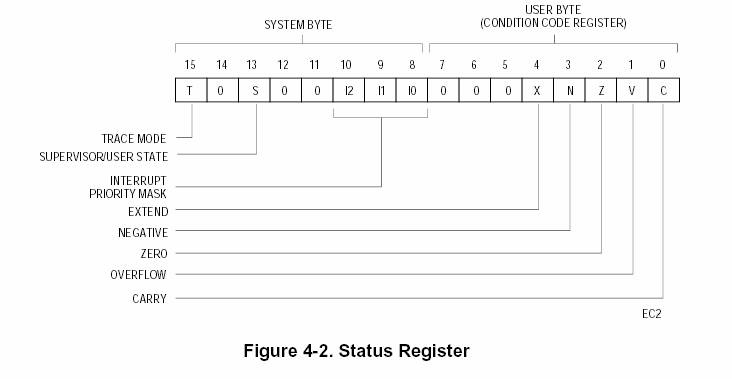
\includegraphics[scale=10,width=1\textwidth]{images/status_register.png}
  \caption{Registro di stato del Motorola68k}
\end{figure}


\subsection{Istruzioni}
Il modello di programmazione è basato su istruzioni. Le istruzioni sono 
composte da:
\begin{itemize}
  \item Codice operativo: indica l'operazione da eseguire;
  \item Operando: indica i dati da usare per l'operazione;
\end{itemize}

In generale, un'istruzione è codificata su un numero variabile di bit che   
dipende dal modo di indirizzamento degli operandi. Infatti, pur essendo di 
16 bit IR (Instruction Register), un'istruzione può essere presa con più 
accessi in memoria.
In particolare, i primi 16 bit dell'istruzione divisi come segue:
\begin{itemize}
  \item 4 bit: codice operativo;
  \item 3 bit: modo di indirizzamento del primo operando;
  \item 3 bit: modo di indirizzamento del secondo operando;
  \item 6 bit: tipo di dato (byte, word, longword);
\end{itemize}

Il grado di efficenza di un'istruzione dipende dal numero di accessi in memoria
effettuati. Per questo motivo, alcune istruzioni sono di lunghezza variabile e 
limitano i modi di indirizzamento che possono avere i due operandi. Ad esempio,
l'istruzione MOVE è di lunghezza variabile e può avere come primo operando solo
un indirizzo di memoria e come secondo operando solo un registro.


\subsubsection{Modi di indirizzamento}
L'indirizzamento è il modo in cui il processore accede ai dati data un'
istruzione. 
In generale, per contenere la lunghezza totale di un'istruzione si usa un 
formato esteso e un formato corto. Il secondo risulta molto più efficiente
del primo e si ottiene limitando il numero di indirizzamenti supportati. Ad 
esempio, nell'istruzione $MOVE$ uno dei due operandi deve essere di tipo 
registro. Di seguito, sono illustrati i quattro tipi di indirizzamento 
supportati dal processore.

\paragraph{Indirizzamento registro}
L'indirizzamento registro è un tipo di indirizzamento molto veloce in quanto 
non richiede l'accesso alla memoria. Il processore, attraverso la sua unità di 
controllo, abilita un registro in lettura e uno in scrittura utilizzando il 
formato corto di un'istruzione specificando con 3 bit il registro sorgente e
con 3 bit il registro destinazione. Inoltre, si ha bisogno di 1 bit per 
indicare se l'operazione interessa un registro $A$ o $D$. Questo tipo di
indirizzamento è molto usato per operazioni in cui ci sono variabili accedute
con molta frequenza. Inoltre, è molto importante notare che, al fine di evitare
conflitti sul registro in scrittura, sul bus del processore ci sono delle 
porte \textit{tristate}.

\paragraph{Indirizzamento immediato}
In questo caso, il valore dell'operando è passato nell'istruzione. Questo è 
particolarmente utile quando si vuole rendere l'istruzione una sola word (16 bit
) per recuperarla in un solo accesso alla memoria. Ad esempio, l'istruzione
$ADD\;\#1,D0$ è molto veloce rispetto ad aggiungere il valore 1 ad una variabile
in memoria.


\paragraph{Indirizzamento diretto}
L'indirizzamento diretto è il più semplice e consiste nel passare l'indirizzo 
della variabile in memoria. Ad esempio, l'istruzione $ADD\;8400,D0$ significa 
aggiungere il contenuto della variabile in memoria \\all'indirizzo 8400 al 
contenuto del registro $D0$. In questo caso, il processore utilizza i registri
$MAR$ e $MDR$ per interfacciarsi con la memoria.

\paragraph{Indirizzamento indiretto}
L'indirizzamento indiretto è molto simile\\ all'indirizzamento diretto. La 
differenza è che il valore dell'indirizzo si trova nei registri $A0$ e quindi 
bisogna leggere il valore dal registro e poi leggerlo dalla memoria. Si tratta 
di un indirizzamento molto lento in quanto richiede due accessi alla memoria ed 
è analogo alla sintassi C $*p$ in cui si accede al valore puntato dal puntatore. 
In assembler, per accedere al valore puntato da un registro $A$ si scrive $(A)$.
Ad esempio per caricare il valore puntato dal registro $A0$ si scrive $MOVE\;(A0)
, D0$. 

\paragraph{Esercizio}
Per ogni istruzione indicare il numero di accessi in memoria effettuati sia
per prendere gli operandi che per prendere l'istruzione.


\begin{center}
\begin{tabular}{ ||c c c ||}
  \hline
  Istruzione & Acc. Mem. Istruzione & Acc. Mem. Operandi \\
  \hline \hline
  MOVE.W D0, D1 & 1 & 0 \\  
  MOVE.B D1, D0 & 1 & 0 \\  
  MOVE.L (A0), (A1) & 1 & 2+2 \\  
  MOVE.L VAR1, VAR2 & 1+2+2 & 2+2 \\  
  CMP.W VAR1, D0 & 1+2 & 1  \\   
  \hline
\end{tabular}
\end{center}
Note: dalla memoria vengono presi 16 bit per volta. Quindi le longword vengono 
prese in 2 accessi.

\subsubsection{Istruzioni di movimentazione dei dati}
Di questa famiglia fanno parte le istruzioni che leggono/scrivono dati da memori
a
e registri.

\paragraph{Move} Questa istruzione
prevede due operandi di cui
il primo è sempre un registro e il secondo può essere uno qualsiasi dei 4 tipi
di indirizzamento ad 
eccezione di quello immediato. La sintassi è $MOVE\;OP1,OP2$. 
L'effetto dell'istruzione è quello di copiare il valore di OP1 nel registro OP2.
Esiste anche l'istruzione MOVEA che è identica alla MOVE ma che non modifica i
flag.

\paragraph{LEA} L'istruzione LEA (Load Effective Address) carica l'indirizzo 
della variabile in memoria nei registri $A$. Ad esempio, l'istruzione $LEA\;VAR 
, A0$ carica l'indirizzo di VAR nel registro $A0$.

\subsubsection{Istruzioni logico-aritmetiche}
Di questa famiglia fanno parte le istruzioni che effettuano operazioni logico-ar
itmetiche.

\paragraph{ADD} L'istruzione ADD prevede due operandi di cui quello destinazione
è sempre un registro mentre quello sorgente può essere uno qualsiasi dei 4 tipi 
di indirizzamento. La sintassi è $ADD\;OP1,OP2$. 
L'effetto dell'istruzione è che il registro OP2 contiene il risultato 
dell'operazione OP1 + OP2. Analogamente, esiste l'istruzione SUB che 
sottrae OP2 a OP1.

\paragraph{CMP} L'istruzione CMP prevede due operandi e non modifica i registri.
La sintassi è $CMP\;OP1,OP2$. In particolare, se il bit $Z$ è a 1 allora $OP1=OP2$
, se il bit $Z$ è a 0 allora $OP1\neq OP2$. Analogamente, se il bit $C$ è a 1 allora 
$OP1<OP2$ e se il bit $C$ è a 0 allora $OP1\geq OP2$.

\subsubsection{Istruzioni di controllo flusso}
Di questa famiglia fanno parte le istruzioni che consentono di modificare l'ordi
ne
di esecuzione delle istruzioni. In particolare, ci sono le istruzioni di salto 
(assoluto o relativo) e quelle di salto condizionale (che utilizzano il bit calc
olato
durante l'istruzione CMP).

\paragraph{BRA} L'istruzione BRA (Branch Always) prevede un solo operando e cons
ente 
di saltare ad un etichetta. La sintassi è $BRA\;\#ETICHETTA$.

\paragraph{BCC} Utilizza i bit CC definiti in precedenza del registro di stato.
Ad esempio può essere usata l'istruzione BNE (Branch Not Equal) che salta se il 
bit Z è a 0.
Oppure l'istruzione BEQ (Branch Equal) che salta se il bit Z è a 1.
Altre istruzioni sono BGE (Branch Greater or Equal) che salta se il bit N è ugua
le al bit V. Di questi codici operativi esistono sia le versioni \textit{unsigned} 
che \textit{signed}.

\paragraph{JMP} L'istruzione JMP (Jump) prevede un solo operando e consente di
saltare in un indirizzo di memoria. La sintassi è $JMP\;OP1$.

\paragraph{JSR} L'istruzione JSR (Jump Subroutine) prevede un solo operando e 
consente di saltare in un indirizzo di memoria. La sintassi è $JSR\;OP1$.
La differenza con l'istruzione JMP è che JSR salva l'indirizzo di ritorno
sullo stack.

\subsubsection{Psuedo-istruzioni}
M68K ha delle istruzioni che non sono codificate in hardware,
ma che sono utili ad altri componenti (come l'assemblatore) per facilitare la
scrittura del codice. Ad esempio, la direttiva ORG permette di specificare 
l'indirizzo di memoria in cui iniziare a scrivere il codice.\\ 
Esistono invece degli operatori che servono a dichiarare le variabili: DC (
Define Constant) e DS. In particolare, DC è un operatore che permette di 
dichiarare una variabile di un certo tipo (byte, word, longword) e di 
assegnare un valore;
DS è un operatore che permette di dichiarare una variabile di un certo tipo
{byte, word, longword} ma non consente di assegnare un valore.\\

Inoltre, se in un programma ci sono variabili il cui valore non cambia, 
è possibile dichiararle come come costanti con la direttiva EQU.

\paragraph{Esercizio: copia di un vettore}
L'esempio che segue si occupa di copiare un vettore di 10 elementi da un array 
in un altro array. Prima di tutto è mostrato il programma in C con
l'utilizzo di puntatori. Successivamente viene mostrato il codice in assembly.


\begin{lstlisting}[caption={Copia di un vettore in C}, language=C]
#include <stdio.h>
int main(void) {
  int a[10] = {0, 1, 2, 3, 4, 5, 6, 7, 8, 9}, b[10];
  int i = 10;
  int *pa, *pb;

  pa = &a[0];
  pb = &b[0];

  while (i--) {
    *pb = *pa;
    pa += 1;
    pb += 1;
  }
  for (i = 0; i < 10; i++) {
    printf("%d ", b[i]);
  }
}
\end{lstlisting}

\begin{lstlisting}[caption={Copia di un vettore in Assembler},language={[Motorol
a68k]Assembler}]

    ORG     $8000 *inizializzo l'area di memoria

    A       DC.B 4,7,2,1 * dichiaro l'array A, di 4 elementi

    ORG     $9000
    B       DS.B N
    N       EQU 4

* inizializzo i puntatori
    LEA     A,A0 
    LEA     B,A1

* Istruzioni equivalenti al LEA
*   MOVEA.L #A,A0 ;il # prende l'indirizzo della variabile e non il valore
*   MOVEA.L #B,A1

* Metto la variabile i nel registro per incrementarla
    MOVE.W #0, D1 * si potrebbe usare l'istruzione RESET

* Comparazione i con N
FOR CMP #N, D1

*  se sono arrivato a N esco
    BGE FINE

* corpo del ciclo
    ADD.W #1, D1 * si potrebbe usare il codice operativo RESET

* copio il valore puntato da A incrementarla
    MOVE.B (A0), (A1) * "()" indica il valore puntato, analogo a "*"

* incremento i puntatori (devo usare aritmetica dei puntatori)
    ADDA.L #1, A0
    ADDA.L #1, A1

* Questa istruzione sostituisce le 3 precedenti.
    * MOVE.B (A0)+, (A1)+ ; utilizzo del puntatore con post incremento

    JMP   FOR

FINE 
LOOP    JMP   LOOP
\end{lstlisting}

L'etichetta FOR è utilizzata per il salto condizionale: ogni volta che viene 
eseguita l'istruzione $CMP$, se il valore di $i$ è minore di $N$, si passa
all'istruzione $ADD.W\;\#1, D1$
che incrementa il valore di $i$. Se il valore di $i$ è maggiore o uguale a $N$, 
si passa al salto condizionale BGE che salta all'etichetta FINE.\\

\subsection{Subroutine}
Le subroutine sono delle funzioni che possono essere chiamate da un programma.
In M68K, le subroutine sono chiamate tramite l'istruzione JSR.\\
L'esempio mostra in un programma che effettua l'operazione $b = a$

\begin{lstlisting}[caption={Copia a in b},language={[Motorola68k]Assembler}]
  ORG         $6000
  MOVEA.L B,  A0  * 6000-6005
  MOVE.W A,   D0  * 6006-6011
  JSR         SUBPRG  * 6012-6017 

  ORG         $7000
  SUBPGR      MOVE.W D0, (A0)
  RTS
\end{lstlisting}

Prima di usare la subroutine è necessario preparare i parametri mettendoli nei 
registri.
In questo caso, il primo parametro è messo nel registro A0 e il secondo 
parametro è messo nel registro D0.\\

Quando arriva a JSR bisogna ricordarsi dove ritornare quando la funzione termina.
L'indirizzo di ritorno (in questo caso 6018) viene salvato sullo stack pointer 
(SP)
in maniera implicita dal codice operativo. Il ripristino del program counter 
(PC) viene fatto automaticamente
dalla subroutine con l'istruzione RTS (Return from Subroutine).\\
I parametri di ingresso possono essere scambiati per valore, mentre quelli di 
uscita
devono essere necessariamente scambiati per riferimento.\\

Questo meccanismo è poco efficiente, perché ogni volta che si chiama una 
funzione
si deve salvare lo stack pointer e ripristinarlo alla fine della funzione. 
Inoltre,
non posso chiamare più di 7 funzioni, perché i registri A0-A6 sono usati per 
passare i parametri.\\

Infatti, si utilizza lo stack per allocare le variabili di un sottoprogramma.
All'inizio dello stack si mettono i parametri di ingresso e alla fine dello 
stack si mettono i parametri di uscita. In generale, per ottenere un valore da 
una funzione esistono due strade:
\begin{itemize}
  \item il valore del risultato viene inserito sullo stack e prelevato dal 
    programma chiamante. In questo caso, il programma chiamante deve riservare 
    dello spazio sullo stack e la funzione deve scrivere il risultato.
  \item la funzione scrive all'indirizzo della variabile di uscita il risultato.
    In questo caso il programma chiamante deve passare l'indirizzo della 
    variabile sullo stack.
\end{itemize}

In questo caso, viene messo prima il valore di A (occuperà 2 byte), poi l'indiri
zzo 
di b (occuperà 4 byte). Infine, c'è l'indirizzo di ritorno (4 byte).\\

Quando la subroutine termina, il valore di A viene ripristinato dallo stack e
viene scritto in b. Quindi dopo RTS si ripristina lo stack pointer,
liberando lo spazio con 
l'istruzione ADDA.L \#6, SP (6 (byte) sono il numero di locazioni sporche).\\

\begin{lstlisting}[caption={Copia a in b passando le variabili sullo stack},
  language={[Motorola68k]Assembler}]

  ORG       $6000
  MOVE.W    A,-(SP)  * metto A nello stack
  MOVE.L    #B,-(SP) * metto l'indirizzo di B nello stack
  JSR       SUBPRG   
  ADDA #6,  SP       * libero lo spazio di memoria

  ORG       $7000
  MOVE.L    4(SP),A0  *ripristino l'indirizzo di B
  MOVE.W    8(SP),D0  *ripristino il valore di A

  SUBPGR MOVE.W D0, (A0)
  RTS
\end{lstlisting}

\subsubsection{Istruzioni LINK e UNLK}
Lo stack può essere utilizzato per salvare i registri che il sottoprogramma 
sporca e allocare variabili locali al suo programma.
In generale, si ha bisogno di due puntatori per sapere dove comincia lo stack 
con i parametri di ingresso e dove cominciano le variabili locali al 
sottoprogramma. Per questo motivo, si introduce un puntatore (Frame Pointer) 
che viene salvato in un registro $A$ attraverso l'istruzione LINK che salva il 
valore vecchio del registro $A$ e incrementa $SP$.

\begin{figure}
  \centering
  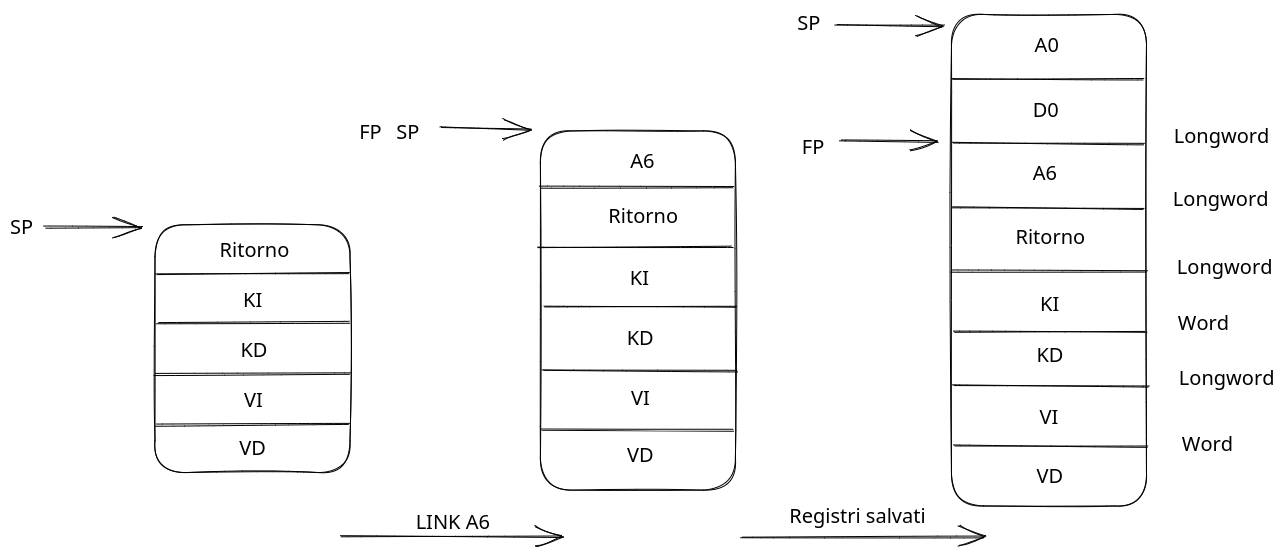
\includegraphics[scale=10,width=1\textwidth]{images/lnk_unlk.png}
  \caption{Diagramma dello stack con le istruzioni LINK e UNLK}
\end{figure}

\begin{lstlisting}[caption={Copia a in b passando le variabili sullo stack},
  language={[Motorola68k]Assembler}]

    ORG       $8000
    VD        DC.W 42 
    VI        DC.W 6
    KD        DS.W 1
    KI        DS.W 1 

    MOVE.W    VD,-(SP)    * metto VD nello stack 
    MOVE.L    #VI,-(SP)   * metto l'indirizzo di VI nello stack 
    ADDA.L    #-2,SP      * riservo lo spazio per KD 
    MOVE.L    #KI,-(SP)   * passo KI per indirizzo

    * salvo i registri
FN  LINK      A6,#0
    MOVE.L    14(A6),A0
    MOVE.W    18(A6),D0
    MOVE.L    DO,-(SP)
    MOVEA.L   A0,-(SP)
    * corpo funzione
    ...
    * ripristino registri 
    MOVEA.L (SP)+,A0 
    MOVE.L  (SP)+,D0
    UNLK    A6
    RTS
\end{lstlisting}


Con questo programma si prende il valore dei registri D0 e A0: prima di effettua
re
l'istruzione JSR, bisogna salvare i registri D0 e A0 nello stack e poi deve esse
re
ripristinato prima di effettuare l'istruzione RTS.\\

Non vogliamo ricordare tutti gli spiazzamenti delle variabili. Quindi possiamo
utilizzare la direttiva EQU per associare lo spiazzamento: SPA EQU 8 SPA EQU 4.

\paragraph{Esercizio: azzeramento di un vettore}

\begin{lstlisting}[caption={Esercizio: carico programmi nello stack},
  language={[Motorola68k]Assembler}]

  ORG     $8000
  N       EQU 50
  VET     DS.B N
  ON      EQU 8
  VET     EQU 4

  * programma principale
  ORG     $7000

  * carico N nello stack
  MOVE.W  #N,-(SP)

  * carico VET nello stack
  MOVE.L  #VET,-(SP)

  JSR     PIPPO

  * cleanup
  ADDA    #6,SP

  * sottoprogramma

ORG     $9000
PIPPO   MOVE.W    ON(SP),D0
        MOVEA.L   OVET(SP), A0
        CLEAR.W   D1 *i cicclo

FOR     CMP       D0, D1
        BGE       FINE

* corpo del ciclo
        MOVE.B #0, (A0)+ *incremento il puntatore

* incremento la variabile di ciclo
        ADD.W #1, D1

        BRA     FOR
FINE    RTS  

\end{lstlisting}

\paragraph{Esercizio: bit alti in una word}
Data una word in ingresso, contare il numero bit di alti in una word
utilizzando un sottoprogramma che conta i bit in un byte.
Per avere più chiaro cosa fare, realizzo prima un programma C.

\lstinputlisting[language=C,caption=Conteggio bit alti in una Word]
{./esercizi/in_classe/bit_count//main.c}

Una prima implementazione con subroutine può essere la seguente. Si noti che non 
c'è il passaggio di parametri tramite stack, ma un accordo tra programma 
principale e funzione sul dove trovare i parametri. Infatti, la il byte
accettato in ingresso dalla funzione viene messo in D0, mentre il risultato
viene messo in D2.


\lstinputlisting[language={[Motorola68k]Assembler},
caption=Bit alti in una Word: versione senza passaggio dei parametri sullo stack]
{./esercizi/in_classe/bit_count/no_stack.asm}

L'implementazione seguente utilizza lo stack per il passaggio dei parametri. 
Si noti come lo stack viene preparato prima di chiamare  la funzione.
Innanzittutto, viene riservata una word per il risultato della funzione,poi 
viene caricato l'indirizzo del vettore delle maschere di bit,  poi la sua
dimensione e infine il il byte da analizzare. Si noti come, la funzione
chiamante utilizza solo  il valore di ritorno dallo stack, in quanto la pulizia
dello stack è fatta dalla funzione stessa. Tutta via però questa 
implementazione non è ottimale, perché la funzione può sporcare i registri che
potrebbero essere in utilizzo da altri programmi.\\ 
Infine, la funzione salva il valore di ritorno nel registro $A1$ e poi utilizza
le costanti $xxxOFF$ per accedere ai parametri passati allo stack.\\

\lstinputlisting[language={[Motorola68k]Assembler},
caption=Bit alti in una Word: versione con passaggio dei parametri sullo stack]
{./esercizi/in_classe/bit_count/with_stack_no_link.asm}


Nell'implementazione precedente, la funzione $COUNT\_FN$ utilizza i registri del 
proessore senza preoccuparsi di salvarli. Questo può causare problemi nel caso 
in cui la funzione venga chiamata da un'altra funzione. Per risolvere questo 
problema, si usa il meccanismo del frame pointer (FP) con l'istruzione $LINK$.\\
Infatti, con il frame pointer si crea una sezione dello stack in cui vengono  
salvati i registri sporcati dalla funzione ottenendo di fatti un'area dati 
locale per il sottoprogramma. Ovviamente, alla fine della funzione deve essere
effettuata la procedura di ripristino.\\ 

\lstinputlisting[language={[Motorola68k]Assembler},
caption=Bit alti in una Word: versione con passaggio dei parametri sullo stack 
e istruzioni LINK/UNLK]
{./esercizi/in_classe/bit_count/main.asm68k}


In particolare, nella versione sopra, si utilizza il registro $A6$ come FP 
attraverso l'istruzione $LINK A6,\#0$ (si inizializza A6 allo stesso valore
dello 
stack). Successivamente, con l'istruzione $MOVEM.L\;D0-D4/A0, -(SP)$, si salvano 
i registri del processore sullo stack. In questo modo è possibile utilizzare
questi 
registri liberamente. Il caricamento delle variabili avviene alla stessa maniera,
facendo riferimento al frame pointer. Si noti però, che gli offset sono stati 
incrementati di 4 perchè l'istruzione $LINK$ salva il valore del registro $A6$ 
sullo stack. Infine, si mette il risultato della funzione in $A6$ e con 
l'istruzione 
duale $MOVEM.L\;(SP)+, D0-D4/A0$ si ripristinano i registri del processore. La 
funzione termina con l'istruzione $UNLK A6$ che ripristina il valore del 
registro 
$A6$ e con l'istruzione $RTS$ che riporta il controllo al programma chiamante.\\


In figura \ref{fig:stack_bit_count}, è riportato il diagramma dello stack dopo
l'esecuzione del programma.

\begin{figure}
  \centering
  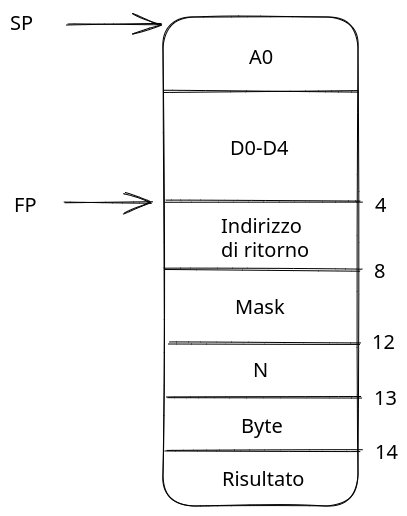
\includegraphics[width=0.5\textwidth]{images/stack_bit_count.png}
  \caption{Diagramma dello stack dopo l'esecuzione del programma}
  \label{fig:stack_bit_count}
\end{figure}

Il programma chiamante con l'istruzione $ADDQ\;\#6,SP$ porta lo stack a puntare al risultato.\\
\paragraph{Esercizio: operazioni sulle matrici}
I dati forniti da un’immagine video vengono memorizzati in una matrice di NxM
byte. 
Definire un programma assembly tramite cui:  
\begin{itemize}
  \item Calcolare il valore di grigi massimo e minimo;
  \item Scambiare la riga contenente il valore massimo con la riga 
    contenente il valore minimo.  
\end{itemize}
Nel caso di una matrice quadrata, contare il numero di bit alti sulla diagonale.

Per semplicità, l'esercizio è stato svolto prima in C ed è mostrato di seguito 

\lstinputlisting[language=C,caption=Esercizio scambio righe di una matrice]
{./esercizi/in_classe/matrix/main.c}

In questo esercizio, si è scelto di passare i parametri di uscita per indirizzo 
invece che utilizzare il loro valore di ritorno. Analogamente alla soluzione 
$C$, il programma $assembly$ è stato scritto in modo da utilizzare funzioni 
simili che saranno riportate di seguito.


\lstinputlisting[language={[Motorola68k]Assembler},
caption=Svolgimento esercizio matrici in assembler]
{./esercizi/in_classe/matrix/main.a68}

Le matrici in assembler vengono rappresentate come array di byte, quindi per 
accedere 
ad un elemento della matrice bisogna basta effettuare un ciclo. In questo caso,
essendo interessati anche alla riga degli elementi massimi e minimi sono 
necessari due cicli annidati per discriminare le righe. Si noti come venga 
passato l'indirizzo delle variabili di uscita nello stack invece di riservare
uno spazio vuoto.
In particolare, il codice si compone di 4 procedure:
\begin{itemize}
  \item COUNT\_FN:\@ conta il numero di bit settati in una matrice e ritorna il 
    risultato
  \item FIND\_MAX:\@ trova il massimo della matrice e ritorna l'indice della
    rigacon i parametri (byte[][] a, int n, int m, int *v, int *r)
  \item FIND\_MIN:\@trova il minimo della matrice e ritorna l'indice della riga
    con i parametri (byte[][] a, int n, int m, int *v, int * r)
  \item SWAP:\@ scambia le righe della matrice passate in ingresso ha una firma 
    del genere void (byte minR[], byte maxR[], int col)
\end{itemize}

Infine, se la matrice è completa viene accumulato il risultato dei bit set nella
diagonale. 

\paragraph{Esercizio: coda}
Sia data una coda e due vettori di supporto. Scorrere gli elementi del vettore 1: 
\begin{itemize}
  \item Per ogni byte pari a 1, effettuare un’operazione di inserimento in coda, 
    inserendo il corrispondente elemento del vettore 2;  
  \item Per ogni byte pari a 0, effettuare un’operazione di prelievo dalla coda.
\end{itemize}

Innanzitutto, è mostrato una soluzione in C, in cui viene dichiarata una
struttura $queue$ con i puntatori testa, coda e un area dati allocata come un 
vettore. Per semplicità la dimensione è stata indicata come statica.

\lstinputlisting[language=C,caption=Implementazione di una coda in C]
{./esercizi/in_classe/queue/main.c}

Mentre di seguito viene mostrata la soluzione in assembler.

\lstinputlisting[language={[Motorola68k]Assembler},
caption=Soluzione in assembler]
{./esercizi/in_classe/queue/main.a68}

\subsection{Architetture parallele}
Il processore visto finora non è efficiente in quanto ogni fase dell'istruzione 

impegna un pezzo dell'architettura. Ci sono diversi modi per avere prestazioni
migliori come ad esempio l'aumentare del clock e  l'aggiunta di più bus.\\

In generale, per avere un aumento di performance bisogna introdurre nel sistema 
un grado di parallelismo che può essere di due tipi: interno (o implicito) e 
esterno
(o esplicito). Le architetture con parallelismo interno sono dotate di un solo 
processore in cui si agisce sull'elaborazione di più istruzioni 
contemporaneamente;
mentre le architetture con parallelismo esterno sono a loro volta divise in: 
\begin{itemize}
  \item architetture multi-processore (o multi-core): con questa dicitura si 
    indicano i sistemi con più processori che comunicano tramite una memoria 
    condivisa.
  \item architetture multi-computer: con questa dicitura si indicano i sistemi 
    con più computer che comunicano tramite una rete di comunicazione. In questo
    caso, ogni nodo di elaborazione ha una propria memoria locale e la
    comunicazione 
    avviene attraverso una rete di interconnessione con una periferica di I/O.
    Il collegamento può essere diretto (collego uno agli altri)
    o indiretto (si utilizzano dispositivi dedicati come \textit{switch}).
\end{itemize}

In generale, le architetture multi-core sono più efficienti delle architetture 
multi-computer quando il numero di nodi è piccolo.

Un'altra classificazione tra le architetture parallele è quella SIMD (Single 
Instructtion Multiple Data) e MIMD (Multiple Instruction Multiple Data).

Le architetture con memoria condivisa si prestano meglio a problemi SIMD.
Questo approccio è molto efficiente per problemi di elaborazione di immagini
ed è tipico delle GPU.

\subsubsection{Architetture Pipelined}
Le architetture pipelined realizzano il parallelismo interno e si basano sull' 
esecuzione di più istruzioni contemporaneamente. In particolare, posizionando 
dei registri tra i diversi stadi dell'istruzione, è possibile fare si che
ciascun stadio possa lavorare su un'istruzione diversa.\\ 
In questo modo, il ritardo massimo di un'istruzione è pari al tempo di
esecuzione del più lento stadio. Ovvero detto $t_i$ il tempo di esecuzione dello 
stadio $i$, il ritardo massimo è pari a $t_{max} = \max t_i$.\\ 

In particolare, si analizza la pipeline a 5 stadi implementata da molte 
architetture come ad esempio il MIPS.\\
Una pipeline può essere realizzata se e solo se si rispettano i seguenti 
vincoli:

\begin{itemize}
  \item Sistema sincrono: ogni stadio deve essere indipendente dagli altri, ma 
    deve evolvere con una base dei tempi comune;
  \item Bisogna separare la memoria di istruzioni da quella di dati. Infatti, 
    prelevando ogni colpo di clock un'istruzione, la memoria di istruzioni deve
    essere più veloce della memoria di dati (si utilizzano delle memorie cache).

    La memoria dati deve essere separata da quella istruzioni per evitare che 
    venga modificata durante l'esecuzione di un'istruzione o che ci siano 
    conflitti;
  \item Le istruzioni devono essere di lunghezza fissa;
\end{itemize} 

La pipeline è costituita da 5 stadi ed è mostrata in figura \ref{fig:pipeline}:
\begin{itemize}
  \item IF(Instruction Fetch): preleva l'istruzione dalla memoria. In questa
    fase è coinvolto il PC (program counter) e un addizionatore con cui sommo 4 
    (prossima istruzione) o un valore relativo per compiere un salto.
    Se volessi fare un salto assoluto andrei a scrivere direttamente nel PC. 
    La scelta tra più valori (in ingresso al PC o all'addizionatore) viene 
    fatta con un multiplexer. Nota: di solito il PC si incremente sempre di 4,
    quando bisogna fare un salto si deve decrementare di 4 e poi si aggiunge
    lo spiazzamento;
  \item ID:decodifica dell'istruzione;
  \item EX:esecuzione dell'istruzione;
  \item MEM:lettura/scrittura della memoria;
  \item WB:scrittura del risultato nei registri.
\end{itemize}

\begin{figure}[h]
  \centering
  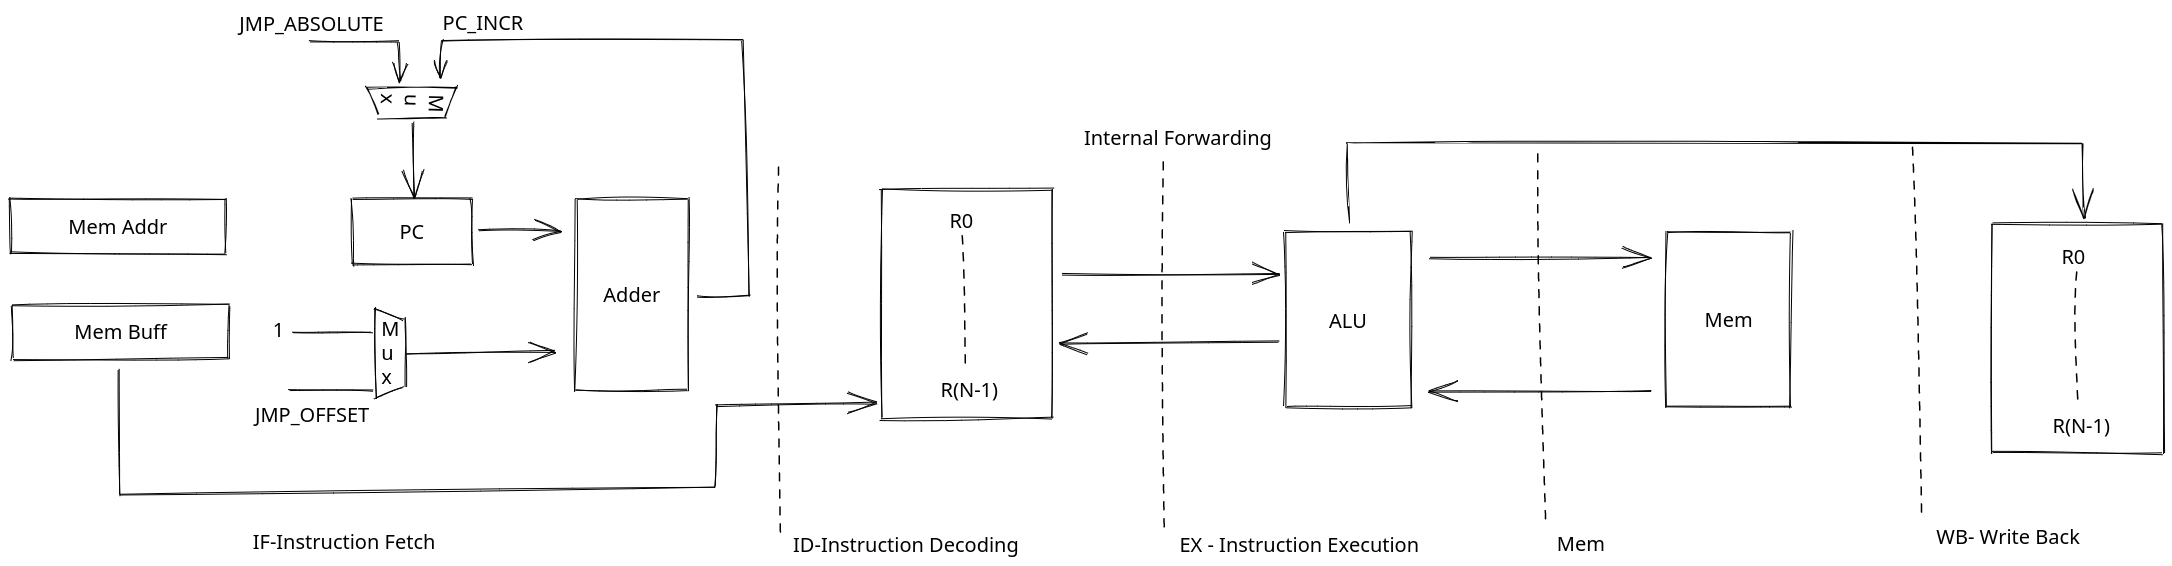
\includegraphics[scale=5, width=\textwidth]{images/pipeline.png}
  \caption{Pipeline a 5 stadi}
  \label{fig:pipeline}
\end{figure}

Per i processori RISC si utilizzano due ipotesi aggiuntive per rendere più
efficiente la pipeline:
\begin{itemize}
  \item Le operazioni aritmetiche devono essere eseguite sempre tra registri. 
    Se così non fosse dovrei andare a prendere gli operandi dalla memoria. 
    Quindi bisogna prima caricare i registri in istruzioni precedenti;
  \item Gli unici modi di indirizzamento consentiti sono immediato e indiretto; 
\end{itemize}

\paragraph{Esempio: istruzioni in pipeline}
Supponiamo di avere due istruzioni in pipeline:\\
$\alpha: R_1 = R_2+ R_3$ e $\beta: R_4 = (R_5)$.\\

Nella fase IF, l'istruzione $\alpha$, con tre operandi, viene prelevata e viene 
caricato il PC con il prossimo indirizzo.\\
Nella fase ID, l'istruzione $\alpha$ viene decodificata attraverso dei registri 
del processore $R_0-R_{15}$.\\ Quindi vengono preparati gli operandi per la fase 
di esecuzione.\\ 
In generale, alla fase di esecuzione basta ricevere il valore di $R_3$ e $R_2$
per fare la somma. Al prossimo stadio bisogna propagare il registro $R_1$
(dove salvare il risultato) e il risultato della somma $R_2 + R_3$.\\
La fase Mem non fa nulla, ma si arriva alla fase WB dove viene scritto il
risultato.

Nell'istruzione $\beta$ ci sono due operandi con indirizzamento indiretto. In 
questo caso nella fase di decodifica si deve andare a prendere il valore di $R_5
$;
la fase esecutiva non fa nulla, ma nella fase Mem viene caricato il valore di
$R_5$.
Infine, la fase WB scrive il risultato nel registro corretto.

Nota: non è possibile caricare 32 bit in una sola istruzione. 
Infatti, se il registro MB è a 32 bit oltre al valore di 32 bisogna codificare
anche il codice operativo.
Esistono delle pseudo-istruzioni che mi permettono di caricare 32 bit in una 
sola istruzione. Sarà l'assemblatore che si occuperà di fare la divisione 
in due istruzioni.\\ 

Le architetture pipelined sono più efficienti laddove i ritardi delle fasi siano
simili. Infatti, si dice che la pipeline è \textbf{bilanciata} se i ritardi delle 
fasi sono uguali. In questo caso, detto $n$ il numero di istruzioni in pipeline, 
il ritardo massimo che si può avere è $\frac{t_i}{n}$.
Nelle architetture pipelined soffrono dei seguenti problemi:
\begin{itemize}
  \item gestione interruzioni: se si verifica un'eccezione durante l'esecuzione 
    di un'istruzione, bisogna fermare l'esecuzione di tutte le istruzioni in 
    pipeline; 
  \item gestione salti: se si verifica un salto, bisogna fermare l'esecuzione di
    tutte le istruzioni in pipeline, invalidare quello che è stato eseguito e 
    modificare il valore del PC. Questo fenomeno è detto \textit{branch penalty};
  \item gestione conflitti per l'accesso in memoria: in questo caso si ha un 
    conflitto tra l'istruzione in esecuzione e quella che deve accedere alla 
    memoria. Questo fenomeno è detto \textit{data hazard};
\end{itemize}

Nella pipeline a 5 stadi, il processore lavora fino a 5 volte più veloce di un 
processore tradizionale. Per questo motivo, è ancora più accentuato il problema 
della comunicazione con la memoria (soprattutto nelle fasi di IF e WB)
che deve essere di tipo cache.\\

Nella tabella di seguito è mostrato il numero di cicli necessari per eseguire 
un'istruzione in un processore pipelined a 5 stadi:
\begin{center}
  \begin{tabular}{|c|c|c|c|c|c|}
    \hline
    \textbf{Istruzione} & \textbf{1} & \textbf{2} & \textbf{3} & \textbf{4} & 
    \textbf{5} \\
    \hline
    \textbf{i-4} & IF & ID & EX & MEM & WB \\
    \textbf{i-3} &  & IF & ID & EX & MEM \\
    \textbf{i-2} &  &  & IF & ID & EX \\
    \textbf{i-1} &  &  &  & IF & ID \\
    \textbf{i} &  &  &  & & ID \\
    \hline
  \end{tabular}
\end{center}

\paragraph{Gestione salti}

Statisticamente, il 30\% delle istruzioni di un programma sono salti. Nel caso 
generale, anche se nella fase ID il processore riconosce un codice operativo di
salto, non può ancora sapere se il salto verrà effettivamente eseguito, in 
quanto dipende dal risultato dell'istruzione in esecuzione. Considerando 
un modello di processore in cui le istruzioni sono a lunghezza fissa, si 
osserva in tabella \ref{tab:branch_penalty} che quando l'istruzione che 
potrebbe generare un salto arriva nella fase $EX$ ($80$), sono state caricate
nella \textit{pipe} anche le successive ($84,88$). Quando si verifica il salto,
bisogna rimuovere queste  ultime istruzioni dalla \textit{pipe} effettuando 
un'operazione di \textit{\textbf{flush}} andando incontro a potenziali ritardi 
ed inefficienze note come  \textbf{branch penalty}. Si nota infatti, come
l'istruzione $88$ viene solo  prelevata, prima di essere scartata e caricare
l'istruzione $100$ (destinazione) del salto.

\begin{figure}
\begin{center}
  \begin{tabular}{|c|c|c|c|c|c|c|c|c|}
    \hline
    \textbf{Istruzione} & \textbf{1} & \textbf{2} & \textbf{3} & \textbf{4} & 
    \textbf{5} & \textbf{6} & \textbf{7}& \textbf{8}\\
    \hline
    \textbf{80} & IF & ID & \textbf{EX} & MEM & WB & & &\\
    \textbf{84} &  & IF & \textbf{ID} & & & & & \\
    \textbf{88} &  &  & \textbf{IF} &  & & & & \\
    \textbf{100} &  &  &  & IF & ID & EX & MEM & WB \\
    \textbf{104} &  &  &  &  & IF & ID & EX & MEM \\
    \hline
  \end{tabular}
  \caption{Andamento pipeline con istruzione di salto}
  \label{tab:branch_penalty}
\end{center}
\end{figure}

Esistono diversi approcci per mitigare il problema del branch penalty:
\begin{itemize}
  \item approccio conservativo: si ferma l'esecuzione di tutte le istruzioni in
    pipeline e si invalida tutto quello che è stato eseguito
    \ref{tab:branch_penalty_cons}. In questo modo, 
    si è sicuri che il salto venga eseguito correttamente. Questo approccio 
    è molto semplice da implementare, ma è molto inefficiente in quanto per 
    ogni salto, si torna, di fatto, al modello sequenziale di Von Neumann 
    (senza alcun grado di parallelismo). Inoltre, in questo caso, la pipeline
    viene svuotata indipendente dal fatto che il salto bisogna effettuarlo o 
    meno. In generale, questo approccio può essere utile nelle architetture 
    RISC perché mettono a disposizione poche istruzioni di salto che possono 
    essere verificate già nella fase di decodifica. Ad esempio, il codice $JNZ$;
    salta se il bit $Z$ del registro di stato è alto;
  \item approccio ottimistico (\textbf{branch prediction}) 
    si tenta di effettuare una previsione su quale ramo del salto verrà eseguito.
    Se la previsione è corretta, si può saltare l'esecuzione di tutte le
    istruzioni in pipeline. Se la previsione è errata, si deve invalidare 
    tutto quello che è stato eseguito. Questo approccio è molto efficiente,
    ma è molto difficile da implementare, in quanto si necessita di un'unità 
    di previsione molto potente;
\end{itemize}

\begin{figure}
  \begin{center}
    \begin{tabular}{|c|c|c|c|c|c|c|c|c|}
      \hline
      \textbf{Istruzione} & \textbf{1} & \textbf{2} & \textbf{3} & \textbf{4} & 
      \textbf{5} & \textbf{6} & \textbf{7}& \textbf{8}\\
      \hline
      \textbf{80} & IF & \textbf{ID} & EX & MEM & WB & & &\\
      \textbf{84} &  & IF & ID & & & & & \\
      \textbf{88} &  &  & &  & & & & \\
      \textbf{100} &  &  &  & IF & ID & EX & MEM & WB \\
      \textbf{104} &  &  &  &  & IF & ID & EX & MEM \\
      \hline
    \end{tabular}
    \caption{Approccio conservativo nella gestione dei salti in architetture 
    pipelined}
    \label{tab:branch_penalty_cons}
  \end{center}
\end{figure}


In generale, esistono due approcci per la branch prediction:
\begin{itemize}
  \item simmetrica: è più semplice da implementare e si basa sull'utilizzo di 
    memorie associative (Branch Prediction Table) che contengono l'indirizzo 
    del branch e l'indirizzo del ramo successivo. Se il branch viene eseguito, 
    l'indirizzo del ramo successivo viene aggiornato. Se il branch non viene 
    eseguito, l'indirizzo del ramo successivo viene aggiornato con l'indirizzo 
    del branch;
  \item asimmetrica:
\end{itemize}

Il predictor è un circuito hardware che si occupa di prevedere dove saltare e 
si basa sull'utilizzo di una memoria associativa. La chiave è l'indirizzo
dell'istruzione di salto. Il valore è l'indirizzo dell'istruzione successiva.\\ 

La memoria associativa è una tabella di indirizzi ed è composta da comparatori
che  sono utilizzati per capire se un dato ci sta o meno. I risultati dei 
comparatori vanno tutti in una $OR$, se questa è alta allora posso guardare
un multiplexer in  cui mi trovo il risultato. Si tratta della stessa tecnologia
usata per la cache con cui viene implementata la memoria istruzioni.
Infatti, ciò è necessaria per avere un tempo di accesso tra istruzioni e
predictor comparabile.\\
Nei cicli, l'errore viene commesso una volta ogni N (condizione di terminazione)
Quindi con la branch prediction non si ottiene un guadagno di prestazioni. 
Infatti, ogni volta che si sbaglia a predirre è anche l'unica. 
Nell'esempio di un doppio for,la predizione diventa dannosa. Infatti, il ciclo
for interno commette l'errore quando esce e quando rientra. Si necessita di un 
sistema più sofisticato che ammetta la possibilità di sbagliare almeno una 
volta.\\ 
Questo problema può essere risolto aggiungendo uno stato a ogni cella della
memoria associativo. Questo sistema a 4 stati è chiamato 
\textbf{2-bit saturating counter} e aggiunge 2 bit alle celle della memoria
associativa. Sostanzialmente, si prende sempre il ramo \textit{than}, al 
primo errore si continua ad andare nello stato \textit{than} ma si aggiorna
lo stato della memoria associativa; al prossimo errore prendo il ramo 
\textit{else}.\\


La branch prediction simmetrica viene implementata attraverso la macchina a 
stati finiti (FSM) di seguito assegnando due bit per lo stato di ciascuna cella 
della memoria associativa.\\

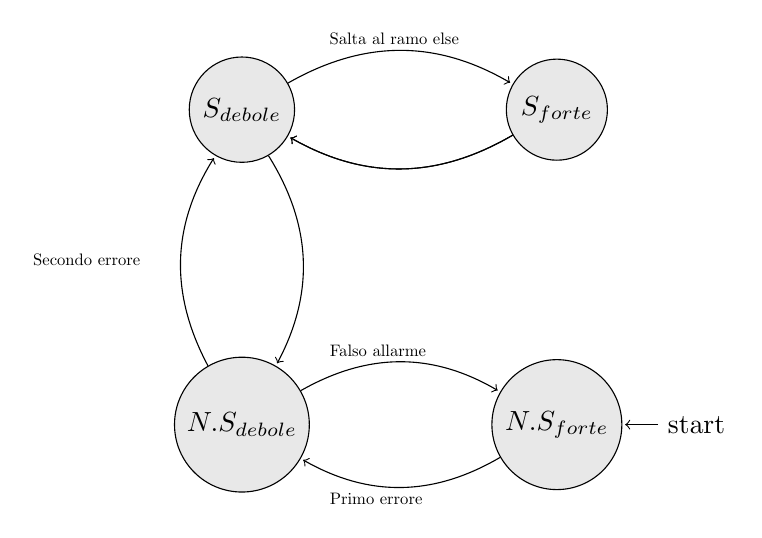
\begin{tikzpicture}[shorten >=1pt,node distance=4cm,on grid,auto]
  \tikzstyle{every state}=[fill={rgb:black,1;white,10}]
  \node[state] (q1) {$S_{debole}$};
  \node[state, right of=q1] (q2) {$S_{forte}$};
  \node[state, below of=q1] (q3) {$N.S_{debole}$};
  \node[state, initial, initial where=right, below of=q2] (q4) {$N.S_{forte}$};
  \path [->] 
    (q2) edge[bend left, above]   (q1)
    (q1) edge[bend left, above] node[text width =3cm, 
      scale=0.6]{Salta al ramo else}(q2)
    (q3) edge[bend left, above]node[text width =3cm, 
      scale=0.6,left]{Secondo errore} (q1)
    (q1) edge[bend left, above] (q3)
    (q2) edge[bend left, above] (q1)
    (q3) edge[bend left, above] node[text width =3cm, 
      scale=0.6]{Falso allarme}(q4)
    (q4) edge[bend left, above] node[text width =3cm, below,
      scale=0.6]{Primo errore} (q3)
    ;
\end{tikzpicture}

Inoltre, la memoria associativa deve essere svuotata. Per farlo si possono 
aggiungere  dei bit di validità aggiornati ogni volta che viene effettuato
un accesso per tenere la pagina più vecchia per applicare un algoritmo di
sostituzione.

\paragraph{Gestione dei conflitti sui dati}
I conflitti possono essere di due tipi:
\begin{itemize}
  \item \textbf{RAW} (Read after write): quando un'istruzione legge un dato
    che è stato scritto da 
    un'altra istruzione che non è ancora stata eseguita;
  \item \textbf{WAR} (write after read): quando un'istruzione scrive un dato
    che è stato letto da un'altra istruzione che non è ancora stata eseguita;
\end{itemize}

\paragraph{Esempio: RAW}
Supponiamo di avere due istruzioni in pipeline:
$\alpha: R_1 = R_2 + R_3$ e $\beta: R_4 = R_1 + R_5$.\\
Bisogna assicurarsi che quando esegue $\beta$ il valore $R_1$ sia corretto. In 
tabella \ref{tab:RAW} è mostrato una pipeline in stallo dove $\beta$
resta bloccata nella fase di decodifica.\\
\begin{table}
  \center
  \begin{tabular}{|c|c|c|c|c|c|}
    \hline
    & 1 & 2 & 3 & 4 & 5\\
    \hline
    $\alpha$ & IF & ID & EX & MEM & WB \\
    \hline
    $\beta$ & & IF & ID & ID & EX \\
    \hline
  \end{tabular}
  \caption{Esempio di RAW}
  \label{tab:RAW}
\end{table}


Quando $\alpha$ finisce la fase di esecuzione $R_1$ diviene il valore che
serve a 
$\beta$. Quando $\beta$ entra nella sua fase di decodifica, il 
valore di $R_1$ è scorretto perchè ancora non è stato scritto in memoria 
($\alpha$ ancora non è arrivata in fase di WB). Questo problema può essere
risolto con la tecnica dell'\textbf{operand forwarding} all'interno dei
processori RISC: quando $\beta$ entra nella fase di decodifica, il valore di
$R_1$ è ancora in $EX$ che lo scrive sia ai registri $R$ della fase precedente 
che in ingresso alla ALU per renderlo disponibile alla fase  successiva 
attraverso un demultiplexer.\\
Quindi, $\beta$ nella sua fase di ID deve sapere che  il valore di $R_1$ deve
prenderlo dalla fase di esecuzione: la fase  esecutiva deve sapere che deve
propagare il valore di $R_1$ alla fase di  decodifica. Quindi nella fase di
esecuzione, c'è bisogno di  un multiplexer che selezioni il valore di $R_1$
da prendere.\\

L'approccio del \textbf{operand forwarding} è ottimale perchè non rallenta il 
processore, ma è applicabile solo ai processori RISC poichè tutte le operazioni
hanno modi di indirizzamento o immediati o diretti. All'interno dei processori 
CISC, invece, non è possibile sapere a priori se l'operando è un registro o una

variabile e nel caso di stallo della pipeline si ha un cache miss che può 
portare 
un accesso in RAM (a causa di un \textit{cache miss})
che rallenta le operazioni di un fattore 10.

Per evitare stalli, nei processori CISC si utilizza la tecnica del
\textbf{internal forwarding}
che consiste nell'ibernare le istruzioni che hanno un conflitto per 
iniziare a segure le successive attraverso delle strutture dette 
\textbf{tabelle di ibernazione}.

\paragraph{Internal forwarding}
Vedere slide sul conflitto dei dati

\subsection{Interruzioni}
Le interruzioni sono un meccanismo che consente al processore di eseguire delle
operazioni senza essere limitato dalla velocità delle periferiche. 
Oltre alla comunicazione cone le periferiche di I/O, le interruzioni sono
utilizzate anche per la gestione dello stato utente e stato supervisore.
Quindi ci sono delle interruzioni che arrivano da unità esterne  
(timer, I/O ecc) altre che arrivano da unità interne e sono dette 
\textbf{eccezioni} (system call, divisione per zero \dots).\\

Nell architetture moderne, le interruzioni possono essere gestite sia in maniera
\textbf{vettorizzata} che \textbf{autovettorizzata}. Con la prima modalità, 
oltre al segnale di interruzione 

Le interruzioni esterne sono analoghe nei processori pipelined e non pipelined. 
Nei sistemi pipelined è importante che l'istruzione che ha generato 
l'interruzione venga eseguita prima di eseguire l'interruzione
(se così non fosse, bisognerebbe 
salvare troppi registri temporanei). Infatti, il processore salva PC
(program counter) e SR (status register) che bastano per ripristinare
l'esecuzione quando l'interruzione viene servita. In particolare,
la fase Instruction Fetch controlla se è arrivata un'interruzione. 
In caso positivo, bisogna aspettare che la pipeline si svuota e poi serve
l'interruzione. In sintesi, le interruzioni esterne sono più semplici da
gestire poichè si generano in un solo punto,mentre quelle interne si generano
in tutte le fasi della pipeline:

\begin{itemize}
  \item Instruction Fetch: accede ad un'area di memoria illegale;
  \item Instruction Decode: codice operativo inesistente o illegale;
  \item Execution: operazioni aritmetiche illegali (divisione per zero);
  \item Memory Access: accesso illegale alla memoria;
  \item Write Back: scrittura illegale in un registro.
\end{itemize}


In generale, il codice operativo di interruzione fa passare il processore in 
stato supervisore e salva il PC e lo SR. Inoltre, avvengono operazioni come 
delimitazione della memoria, spostamento dei registri ecc. Ad esempio, il 
motorola 68000 mantiene un registro $A_7'$ in cui si trova un puntatore al suo
stack che è diverso da quello in fase utente.

\subsubsection{Interruzioni interne}
Le interruzione interne hanno il vantaggio di essere relativamente predicibili.
Infatti, il processore conosce se ha diviso per zero se ha fatto un accesso o
ha effettuato una system call, ma non è possibile conoscere, ad esempio, quando
si verifica un \textit{page fault}.\\

Il processore mantiene una tabella al suo interno in cui ad ogni evento 
corrisponde l'indirizzo della sua $ISR$. Questa tabella sarà popolata in 
fase di configurazione del sistema.

\begin{table}
  \center
  \begin{tabular}{|c|c|c|c|c|}
    \hline
    IF & ID & EX & MEM & WB\\
    \hline
    $i+4$ & $i + 3$ & $i+2$ & $i+1$ & $i$\\
    \hline
  \end{tabular}
  \caption{Istruzioni in pipeline}
  \label{tab:int_pipeline}
\end{table}

In generale, le architetture RISC complesse rinunciano ad avere interruzioni 
precise. Infatti, al verificarsi di un'interruzione interna le istruzioni 
possono essere eseguite non necessariamente in ordine. Seguendo quest'approccio, 
i processori rimandano al software il controllo di correttezza della sequenza 
di istruzioni. Mentre, un altro approccio (più complicato) è quello in cui 
nonostante le istruzioni out of order vengono ricostruite o con approccio
ottimistico o con quello conservativo. Con il secondo, la pipeline viene
invalidata e si procede con l'esecuzione sequenziale di istruzioni
(non c'è parallelismo) fino a quando non si trova l'istruzione che genera
l'interruzione. Nell'approccio ottimistico si procede in pipeline ma si mettono
in piedi meccanismi di roll-back laddove ci fosse un interruzione.
Questi meccanismi sono:

\begin{itemize}
  \item \textbf{Tecnica di checkpoint}: il processore salva tutti i registri 
    del processore (compreso Program Counter) in un'area di memoria (facendo 
    delle fotografie). Quando si verifica un'interruzione il processore
    ripristina i valori dell'ultimo checkpoint e prosegue ad un'istruzione 
    per volta. Ad esempio, date le istruzioni $i: R_4 = R_1$ $i+1: R2 = R0+R6$ 
    $i+2: R_3 = R_1/R_5$. Partendo da uno stato sicuro, si effettua un primo 
    checkpoint e si eseguono le istruzioni. Supponendo che la $i+1$ genera 
    un'eccezione, i registri $R_3$ e $R_4$ vengono ripristinati dal checkpoint;
  \item \textbf{Tecnica di buffer}: il processore salva le istruzioni 
    in esecuzione (inclusi gli operandi) in un'area di memoria. Ogni istruzione
    memorizzata può essere rimossa se e solo se tutte quelle che la precedono
    non generano eccezioni. Quando invece un'istruzione genera un'eccezione si 
    eseguono delle operazioni di UNDO che sono già state eseguite.
\end{itemize}

\subsubsection{Interruzioni nel motorola 68000}
Per potere utilizzare le interruzioni sono necessarie almeno 2 modalità utente in 
quanto ogni volta che bisogna eseguire una ISR bisogna:
\begin{itemize}
  \item salvare il contesto del processore: registri, stato e program counter;
  \item sostituire il program counter con l'indirizzo della ISR;
\end{itemize}

Inoltre, alla fine della ISR bisogna ripristinare l'esecuzione della routine
precedente in maniera trasparente. Per risolvere questo problema, M68K prevede due modalità di 
esecuzione utente e supervisore (discriminate dal bit $S$ del registro di stato).

Quindi, una ISR può essere esguita passando da stato utente a stato supervisore e 
abilitando le interruzioni attraverso i bit $8-10$ del registro di stato detti $IPL$
\textit{interrupt-request priority level} . In particolare, sono disponibili 8 
livelli di interruzione in cui il codice $0$ corrisponde a interrupt disabilitate
e $7$ interrupt non mascherabile. Quindi i livelli codificabili sono da $1$ a $6$.

\subsection{MIPS}

\subsubsection{MIPS assembler}
Il MIPS ha dei registri general purpose. Esiste una convenzione per usarli. 
Bisogna capire come strutturare il codice: area dati e area testo.
Caricare l'indirizzo di un vettore è complicato perchè il mips supporta 16 bit 
invece l'istruzione è a 32. Si usano quindi le pseudo-istruzioni che risoolvono 
in un più istruzioni (una che carica la parte più significativa, una la meno 
significativa e una che li mette insieme); bisogna ricordarsi che quindi la 
pseudo-istruzione $LA$ (load address) prende 2 registri (non possono essere 
utilizzati da altre operazioni). Invece carico un byte con $LB$
Il salto fatto in $BNE$ potrebbe essere un'unica istruzione quando il confronto 
viene fatto tra due registri del processore e il salto relativo si va in una sola 
istruzione.

Esiste un modo per stampare il risultato attraverso il sistema di syscall.
PRima di usare $syscall$ bisogna caricare i registri $A_0$ con il dato da stampare 
e $v_0$ con $4$ (ovvero codice operativo per la syscall da usare. $4$ sta per stampa, 
$10$ sta per exit).
\subsubsection{Pipeline nel MIPS}
La pipeline ha 5 stati. Ha una cache per i dati e una per le istruzioni.
Perchè funziona la pipe nonostante i conflitti? Si può fare l'internal forwarding 
negli stadi 4-5 (esecuzione e scrittura in memoria). Bisogna studiare l'assembler 
per capire l'architettura (nelle slide ci sono gli esempi dei codici operativi )

\subsection{Architettura ARM}
ARM è una specifica di progetto che ognuno può customizzare.

\clearpage
\section{Input/Output}
Comunicare con un dispositivo di I/O equivale a scambiarsi informazioni di 3 tipi: dati,
controllo e stato. Per questo motivo l'interfacciamento verso un dispositivo periferico 
(che sia di input o di output) è composta da tre tipi registri fondamentali:
\begin{itemize}
  \item Registro dato: contiene le informazioni da inviare o ricevere e quindi 
    di conseguenza, sarà predisposto in lettura o in scrittura;
  \item Registro di controllo: utilizzato dall'unità centrale per configurare
    la periferica e/o inviare comandi;
  \item Registro di stato: utilizzato dalla periferico per comunicare eventi 
    che saranno consumati dall'unità centrale;
\end{itemize}

Oltre alla modalità con cui comunicano i due dispositivi, si ha bisogno di un 
set di regole che danno una semantica ai messaggi inviati. Si parla di 
protocolli che si dividino in tre tipologie:

\begin{itemize}
  \item Asincrono: le due entità non hanno un riferimento temporale,
    ma comunicano attraverso segnali. 
    Fanno parte di questa famiglia i protocolli basati su handshaking;
  \item Sincrono: le due entità sono legate da un vincolo temporale. I due 
    sistemi hanno bisogno di un riferimento comune e,pertanto, questo tipo di 
    protocolli sono detti isocroni;
  \item Semi-sincrono: le entità utilizzano dei sistemi di segnalazione, ma 
    trasmettono costantemente dati;
\end{itemize}

\paragraph{Standard nelle comunicazioni}
Nei sistemi di comunicazione standard, alcuni registri vengono utilizzati per 
collegare i terminali delle periferiche (dati, controllo,stato). Di fatto, 
leggendo e scrivendo su queste memorie, avviene la comunicazione. Dal punto di 
vista elettronico, questi collegamenti implementano delle interfacce standard 
indipendendenti dalla tipologia di dispositivo o applicazione. La parte 
software che utilizza queste interfacce è detta driver. Infine, possono 
esistere altre componenti detti adattatori che non aggiungono logica alla 
comunicazione ma si occupano di aspetti elettronici (conversioni di segnali,
di potenza, \dots).\\ 

Dal punto di vista dell'utilizzatore, le periferiche sono viste come un insieme di registri 
speciali in cui scrivendo e leggendo si attivano dei comportamenti "speciali" da parte 
dell'hardware. Il programma che interagisce con questi registri è detto \textit{driver}. 
Nel corso degli anni, per facilitare la scrittura dei driver, le interfacce (ovvero i registri)
che espongono le periferiche sono standard e astraggono la natura hardware (elettro-meccanica)
dei dispositivi. In un sistema in cui sono presenti diversi dispositivi di I/O, diversi 
processori bisogna risolvere due problemi:
\begin{itemize}
  \item invio/ricezione dei dati: implementare dei protocolli per la comunicazione tra due
  dispositivi. Questo punto si risolve aggiungendo dei segnali di controllo alle linee dato 
  che servono a regolare l'attività di invio-ricezione;
  \item gestione delle interruzioni da più periferiche: assumendo di realizzare un sistema 
  \textit{interrupt-based} bisogna conoscere la periferica interrompente per eseguire l'azione
  giusta (\textit{Interrupt service routine}).
\end{itemize}

\paragraph{Esercizio: periferica ideale}
La periferica ideale presa in esame è composta da registri dato, controllo e 
stato e ha un solo modo di funzionamento. Inoltre, come primo esempio si 
suppone che il sistema abbia una sola periferica e si suppone di avere 
la $ISR$ in un'area fissa.
In generale, la struttura di un programma che include I/O è la seguente:
\begin{itemize}
  \item Area periferica: area del programma in cui è allocata la periferica
    (in cui sono collocati i registri dato, controllo e stato);
  \item Area programma principale: programma in cui si configura e avvia 
    la periferica, si abilitano le interruzioni e si svolgono le operazioni 
    come di consueto;
  \item Area interruzioni: funzione che si occupa di gestire l'interruzione;
\end{itemize}

L'esercizio richiede di leggere 100 caratteri dalla periferica. A scopo 
semplificativo, viene riportato una prima versione del programma in 
cui si legge un solo carattere che utilizza la tecnica del \textit{polling}.

\begin{lstlisting}[language={[Motorola68k]Assembler},caption="Lettura 
  1 carattere in polling"]
    * area periferica
		ORG 		$2000 
    DATO    DS.B  1  
    CONT    DS.B  1
    STATO   DS.B  1

    * area main
    ORG     $8000
    MOVE.B  #00000000b,STATO  * reset stato
    MOVE.B  #00000000b,CONT   * reset controllo 
    MOVE.B  #10000000b,CONT   * abilitazione macchina

    *polling: aspetto che lo stato diventi 1
L1  MOVE.B  STATO,D0          * lettura del registro di stato 
    AND.B   #000000001b,D0    * controllo stato
    BNE     L1                * stato == 0 -> polling

    *polling: aspetto che lo stato diventi 0 
L2  MOVE.B  STATO,D0          * lettura del registro di stato
    AND.B   #000000001b,D0    * controllo stato 
    BEQ     L2                * stato == 1 -> polling

    * dato disponibile
    MOVE.B  DATO,D1
    MOVE.B  #00000000b,CONT   * disattivazione periferica
\end{lstlisting}

Il programma risulta poco flessibile e monopolizza la CPU. Un primo 
miglioramento consiste nell'usare l'indirizzamento indiretto e accedere 
ai registri della periferica con i registri $A_i$, Di seguito, si propone un
approccio basato sulle interruzioni. In generale, il meccanismo di 
configurazione della periferica è analogo, eccetto che  in questo caso bisogna
configurarla per lavorare su interruzioni. Infine, sono necessari di 
una variabili risultato e di un contatore per l'esercizio.

\begin{lstlisting}[language={[Motorola68k]Assembler},caption="Lettura 
  100 caratteri con interruzione"]
		ORG 		$2000 
    DATO    DS.B  1  
    CONT    DS.B  1
    STATO   DS.B  1

    ORG     $8000

    * abilitazione della periferica
    MOVEA.L #STATO,A2
    MOVEA.L #CONT,A1
    MOVEA.L #DATO,A0
    MOVEA.L #BUFF,A3
    MOVE.B  #100,CC

    MOVE.B  #00000000b,(A2) * reset stato
    MOVE.B  #00000000b,(A1)
    ABILISR                 * abilitazione delle interruzioni
    MOVE.B  #10000000b,(A1)

    * ISR
    ORG     $3000
    * salva i registri (LINK)
    MOVE.B  (A0),D1
    MOVE.B  #00000000b,(A1)

    * ripristina i registri (UNLK)
    RTE                   * ritorno
\end{lstlisting}

Quando si ha un'interruzione bisogna avere, dal punto di vista hardware, due 
informazioni: chi ha interrotto e il segnale di interruzione. Innanzitutto,
bisogna effettuare una distinzione tra ruolo  dell'hardware e ruolo del 
software.

In generale, per avere più periferiche bisogna avere un PIC che identifica chi
ha interrotto il processore. Il Motorola68k può operare in operare in maniera 
autovettorizzata (3 bit nel registro di stato) o in maniera vettorizzata in  
cui si utilizza il bus dati (8 bit) per mappare le interruzioni.

\begin{figure}
  \centering
  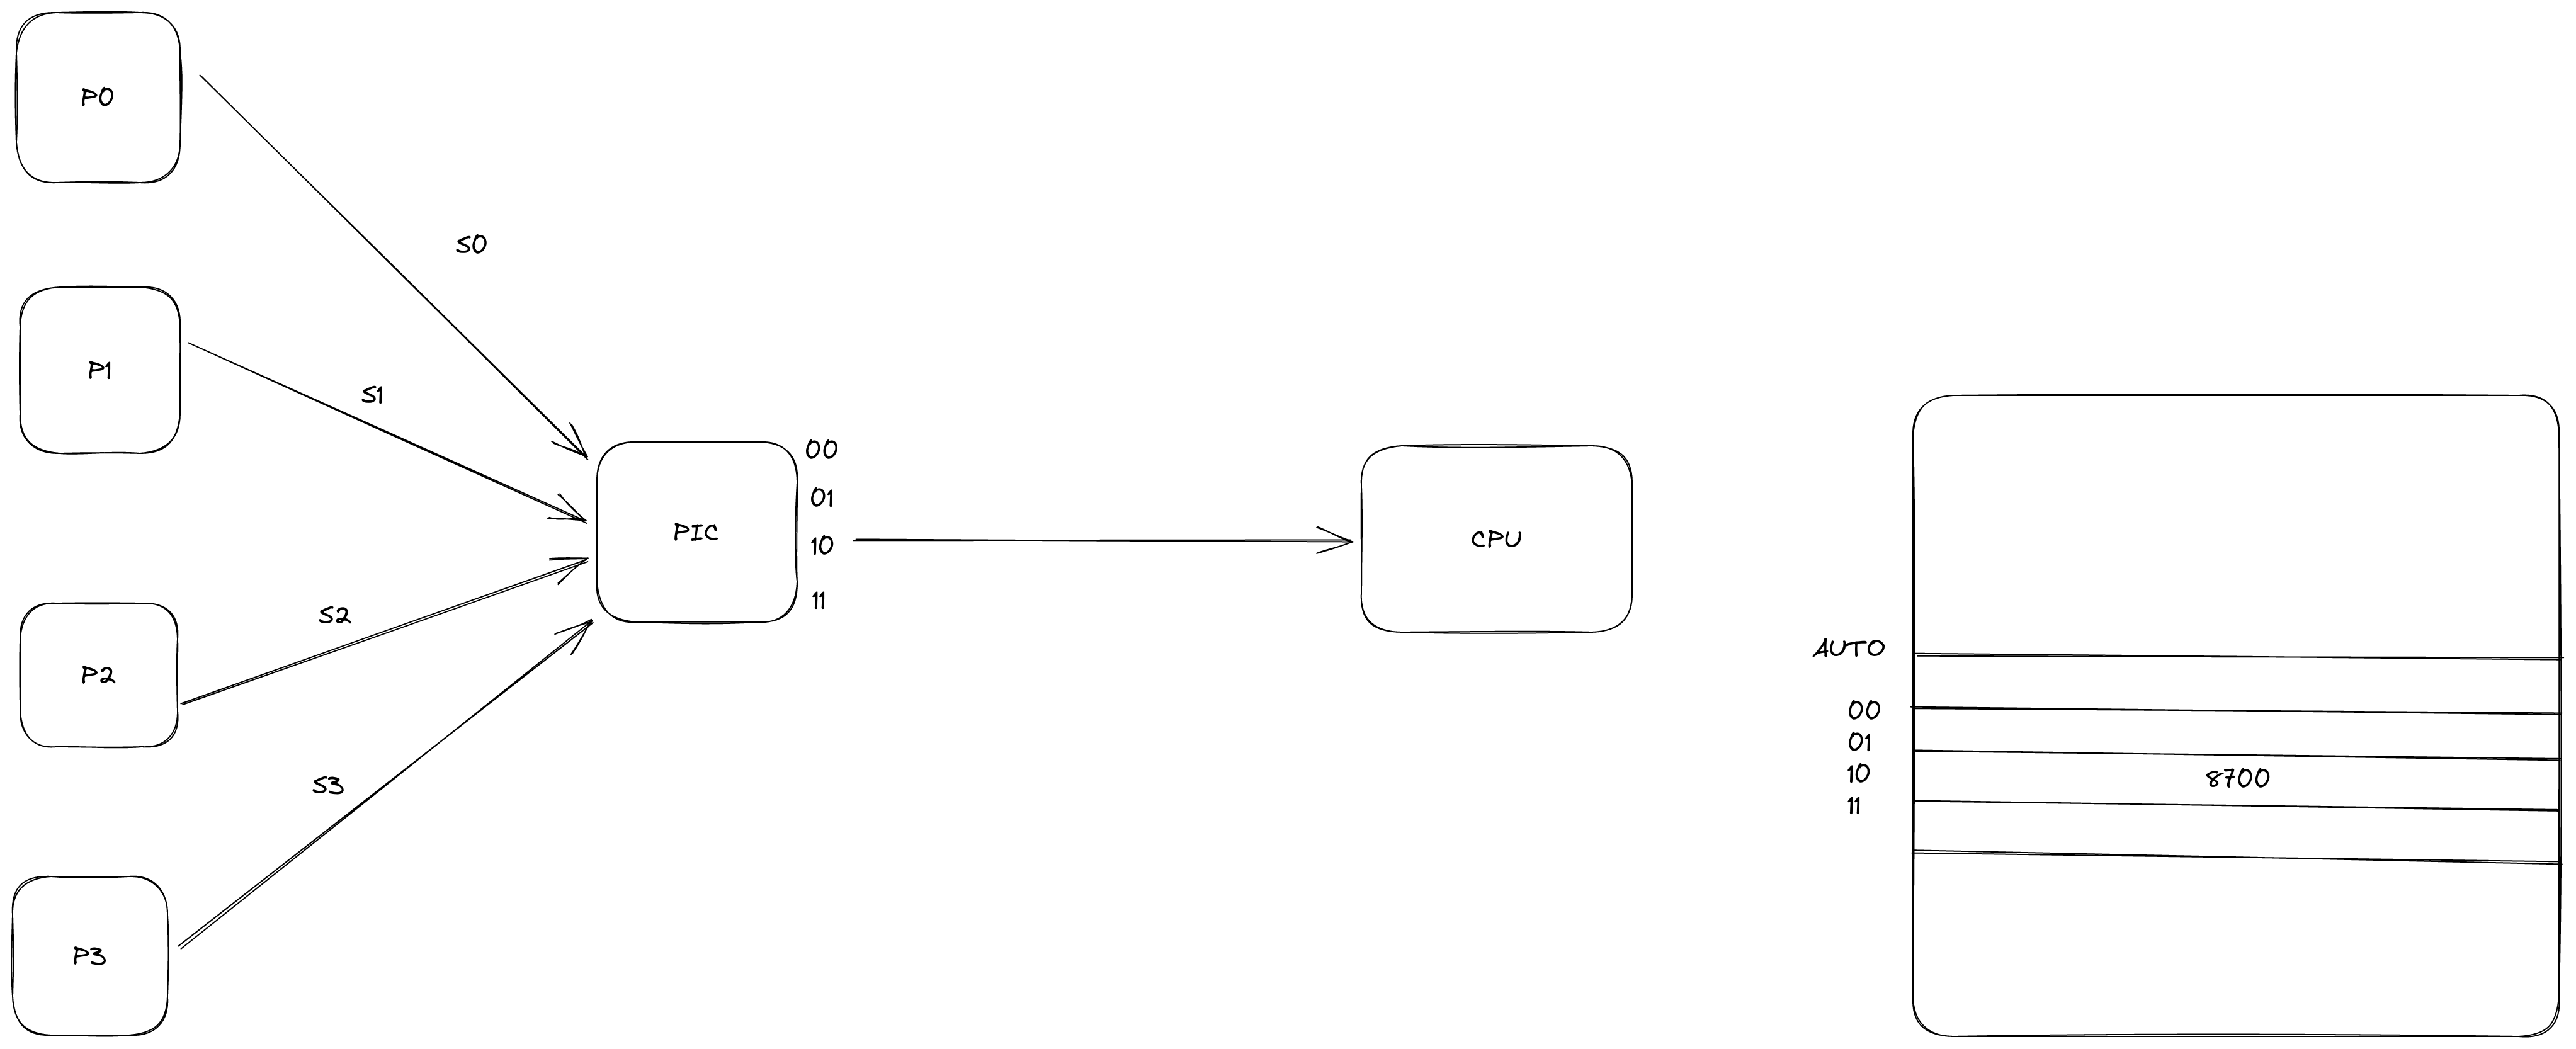
\includegraphics[scale=0.7,width=1\textwidth]{images/architettura_pic.png}
  \caption{Architettura interruzioni con PIC}
\end{figure}

Le interruzioni autovettorizzate sono mappate in un'area di memoria fissa in
cui ad ogni codice di periferica l'indirizzo della ISR corrispondente. In
questo modo quando arriva l'interruzione, il processore deve cambiare il suo
program counter atomicamente (non può essere interrotto) con l'indirizzo della
routine da eseguire.

\subsection{Periferica parallela - PIA Intel MC6821}
Sia dato il problema in cui $B$ voglia inviare un messaggio ad $A$. Si 
suppone di essere in architettura multi-computer (i due sistemi non hanno 
memoria condivisa)e che, per ipotesi, la comunicazione avvenga attraverso un collegamento  parallelo. Il collegamento in parallelo ha bisogno dello scambio  dei segnali di \textit{strobe} per scandire l'invio e la ricezione di ciascun dato. In particolare, la periferica  prevede i seguenti registri:

\begin{itemize}
  \item Dato: può essere utilizzato in input e in output;
  \item Direzione: configura i bit in ingresso o in uscita. In realtà, questo 
    registro viene utilizzato in mutua esclusione con il dato. Fisicamente, 
    infatti dato e direzione sono lo stesso registro discriminati da un bit 
    nel registro di modo;
  \item Modo: il modo serve a configurare la periferica una volta per tutte 
    all'avvio dell'applicazione. Ad esempio, un bit serve a capire se i valori 
    nel registro dato sono effettivamente informazioni da trasmettere oppure 
    configurare i bit in uscita o in ingresso. In questo registro sono
    configurabili $CB_1$, $CB_2$, $CA_1$, $CA_2$. In particolare, per ogni 
    valore bisogna decidere se questo genera o meno un'interruzione e il fronte 
    dei segnali su cui si opera.
\end{itemize}

La periferica è dotata di 2 porti: A usato per ricevere, B usato a cui sono collegati le due coppie di segnali $CA_1, CA_2, CB_1, CB_2$. In particolare, per far comunicare 2 dispositivi il porto $A$ del ricevente deve essere inviata la porto $B$ del mittente. In particolare, il segnale $CB_2$ del mittente è collegato a $CA_1$ del ricevente; mentre $CA_2$ del ricevente è collegata a $CB_1$ del mittente. 

\subsubsection{Protocollo di handshaking PIA}
Nel modo di funzionamento $100$ (bit $5-3$ del registro di controllo), la PIA segue il protocollo di handshaking secondo cui, se $B$ vuole inviare un dato e $A$ vuole riceverlo, funziona nel modo seguente:
\begin{itemize}
  \item B scrive il dato da inviare nel registro dato e abbassa $CB_2$ che, a causa del collegamento diretto, abbassa $CA_1$ del ricevente;
  \item $A$ vede il suo $CA_1$ abbassato e, dato che $CA_2$ lavora in opposizione si alza;
  \item sul segnale $CA_2$ è collegato il bit $CRA_7$ a cui è collegata una linea di interrupt $IRQA$ che genera un'interruzione hardware che deve essere servita dal processore di $A$;
  \item una volta effettuata la lettura, $A$ abbassa $IRQA$, abbassando $CA_2$ e, quindi, abbassando $CB_1$ (sul nodo che trasmette $B$).
  \item L'abbassamento di $CB_1$ comporta l'alzamento di $CB_2$, quindi l'alzamento del bit $CRB_7$ con corrispondente generazione dell'interrupt sulla linea $IRQB$.
\end{itemize}

\begin{figure}
  \centering
  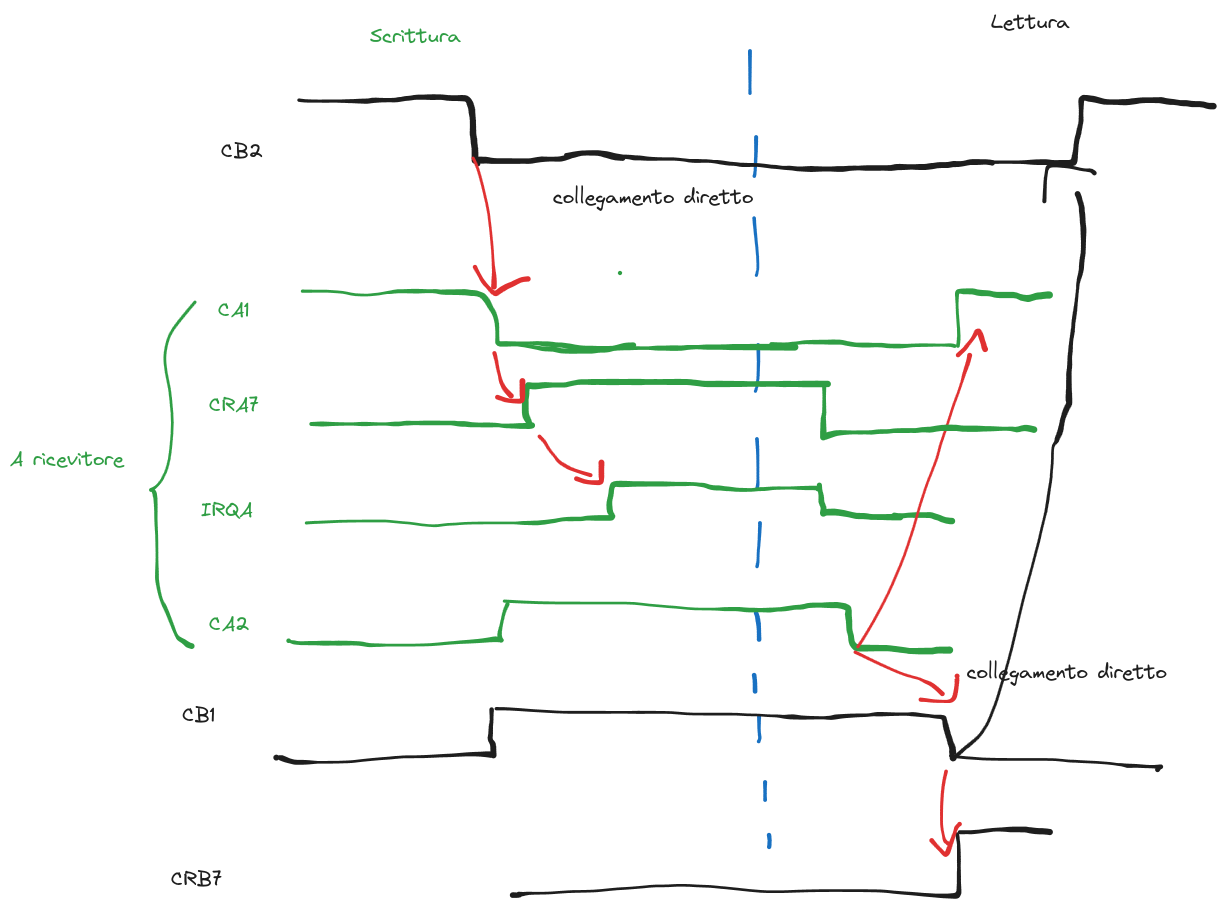
\includegraphics[scale=0.5,width=1\textwidth]{images/pia_handshaking.png}
  \caption{Handshaking comunicazione parallela}
\end{figure}

\subsubsection{Configurazione PIA}
La configurazione delle PIA avviene in due fasi:
\begin{itemize}
  \item invio o ricezione;
  \item configurazione del protocollo di handshaking e interrupt;
\end{itemize}

In generale, la periferica è mappata in registri contigui ($2004$ a $2007$) così disposti come nella figura che segue.

\begin{figure}
  \centering
  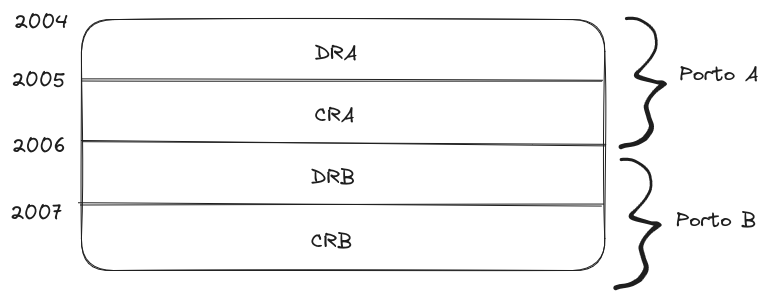
\includegraphics[scale=0.5,width=1\textwidth]{images/mapping_pia.png}
  \caption{}
\end{figure}

\clearpage

\subsection{Periferica seriale}
Per ogni carattere inviato, bisogna effettuare il protocollo per segnalare. In 
generale, le ISR sono uguali la differenza sta nel funzionamento dei due  
dispositivi: la parallela effettua l'handshaking ad ogni carattere (non c'è 
modo di distinguere da un carattere da un altro), la seriale invece dopo 
avere configurato le velocità di invio dei dati (baud rate) può inviare 
continuamente dati in quanto alla fine del protocollo la linea si riporto nello
stato di riposo (1-attivo nel caso della seriale).

\subsection{Mutua esclusione}
In generale, non è possibile disabilitare le interruzioni per garantire l'
atomicità delle operazioni in un sistema complesso. Per questo motivo, si 
utilizzano le aree in mutua esclusione.

Codice TAS (Test and Set) permette di effettuare le operazioni in modo atomico 
senza essere interrotti. Bisogna ricordarsi di segnalare che si ha finito di 
utilizzare la sezione critica in modo tale da sbloccare gli altri processi in 
attesa.

\begin{itemize}
  \item se il bit è zero lo mette a 1 (si può accedere alla sezione critica);
  \item se il bit è 1 allora non si fa nulla
    (non si può accedere alla sezione critica);
\end {itemize}

\begin{figure}
  \centering
  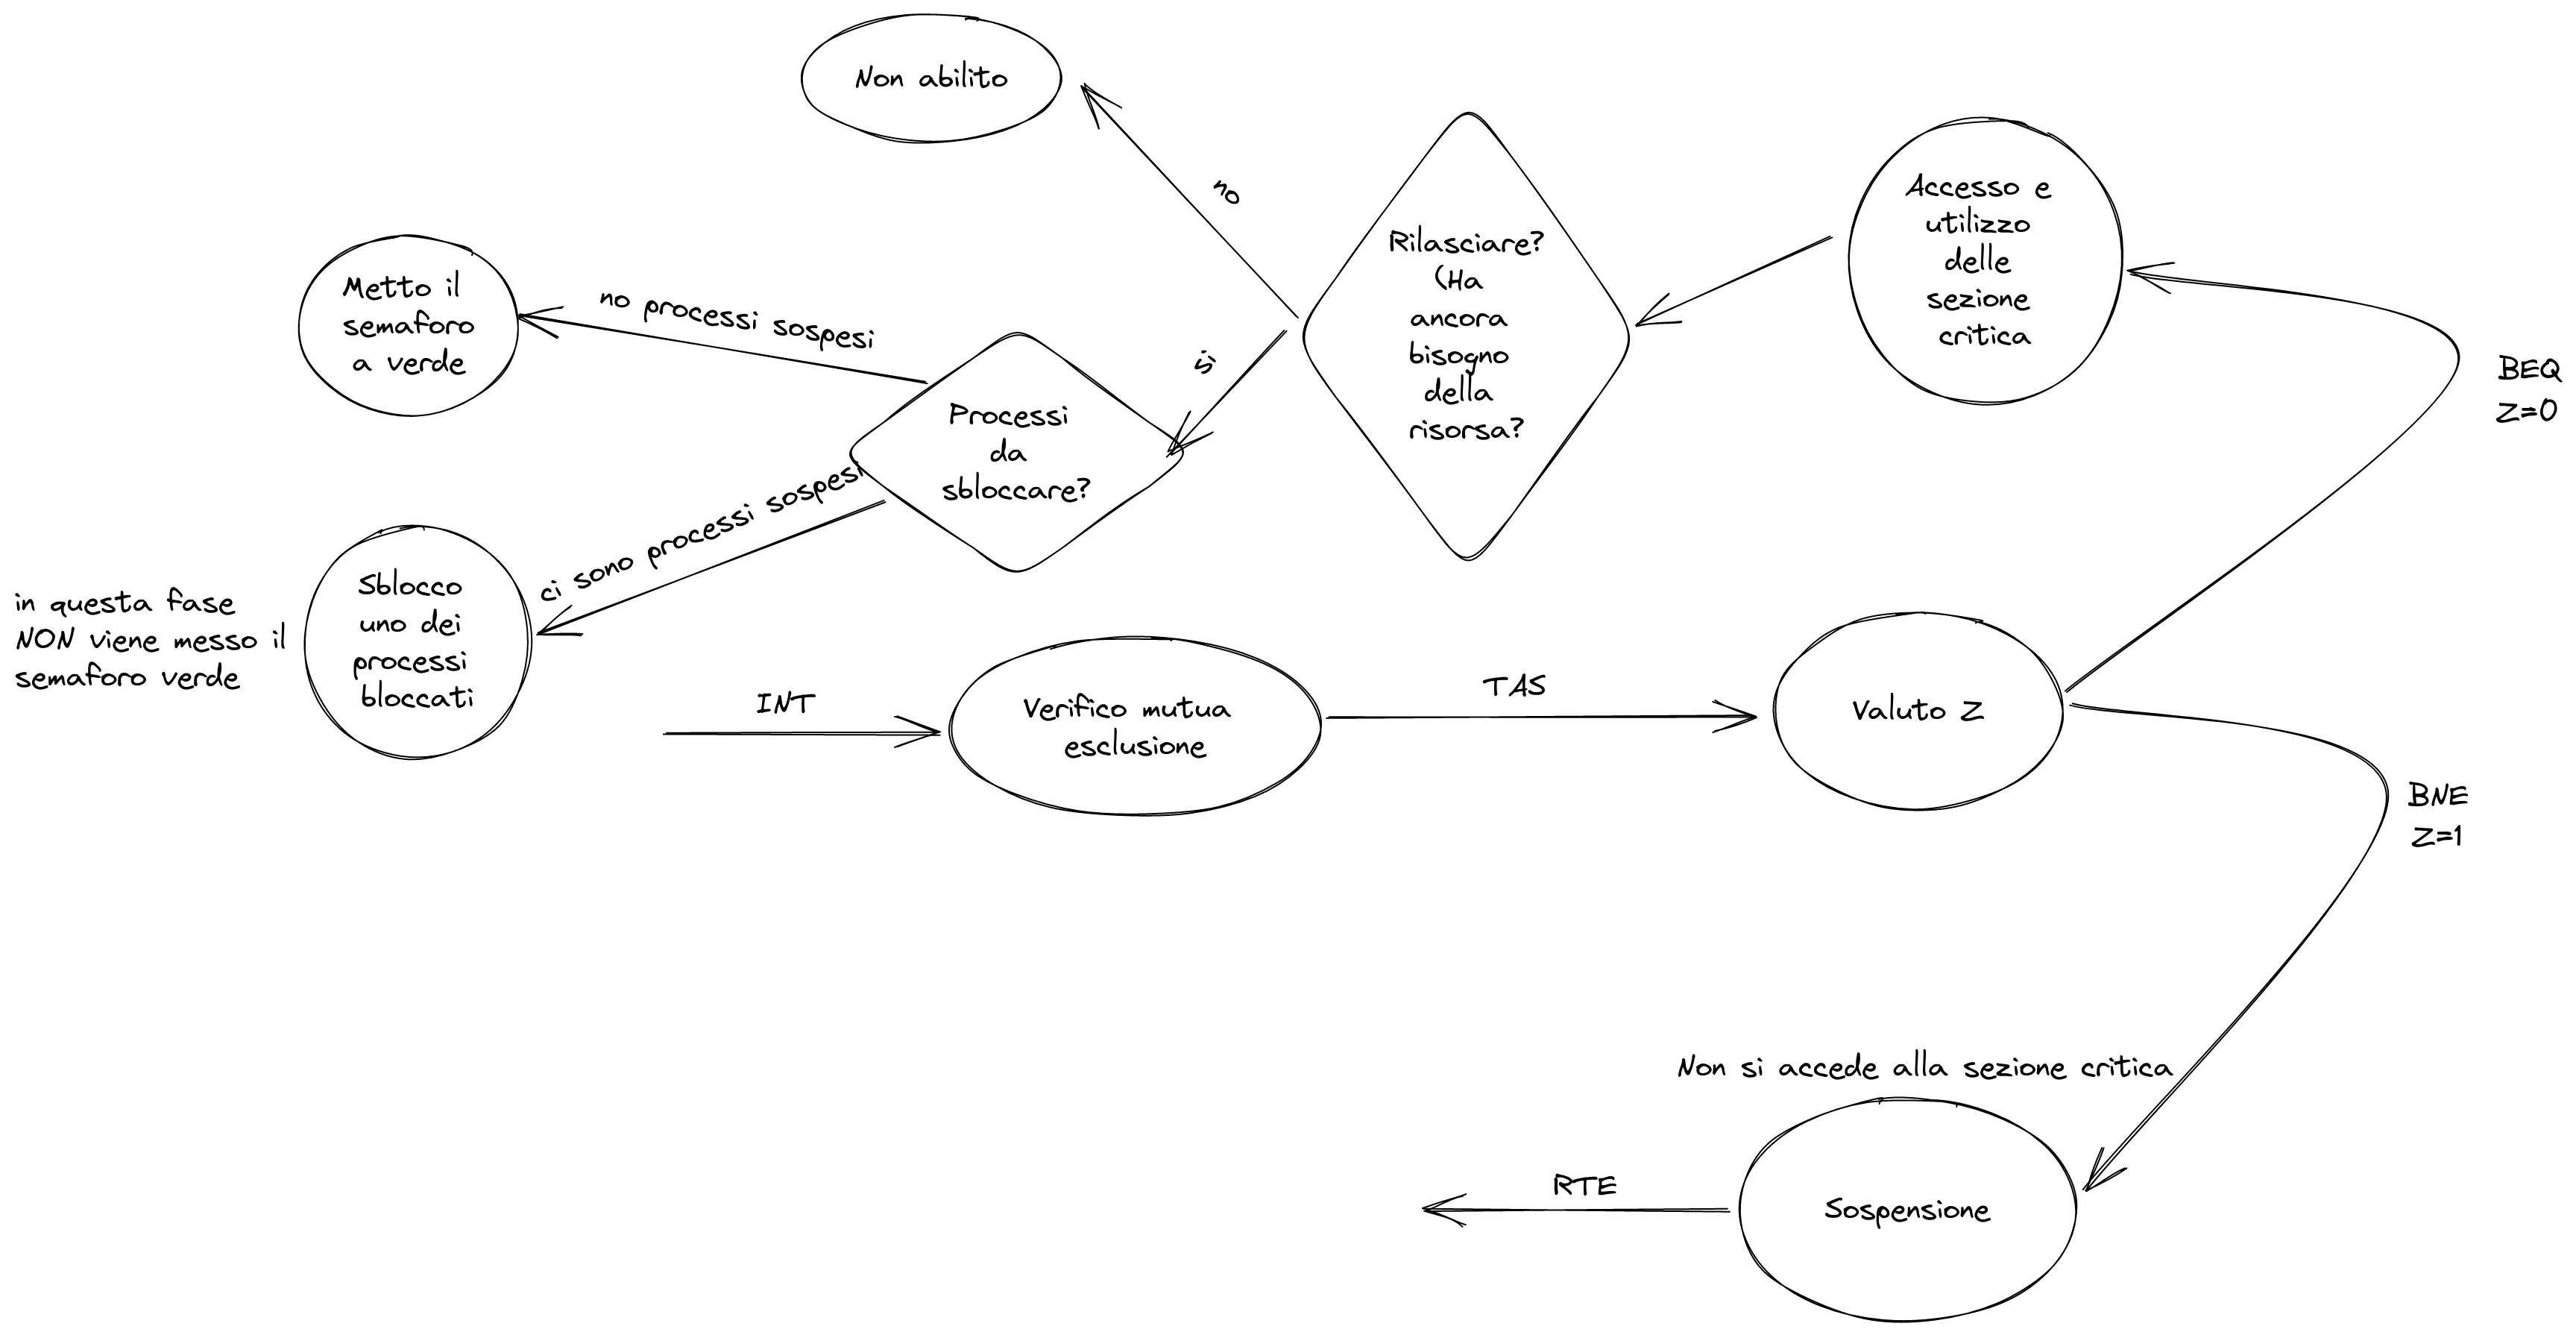
\includegraphics[scale=0.5,width=1\textwidth]
    {images/fsm_critica.png}
  \caption{Automa a stati finiti}
  \label{fig:fsm_critica}
\end{figure}


Per indicare che un processo si trova all'interno di una sezione critica, si 
utilizza una variabile di possesso che è cambiabile solo da chi si trova all 
interno della regione di mutua esclusione; mentre può essere letta dagli altri 
per capire se si possono effettuare le operazioni di scrittura.\\

Per testare, bisogna assegnare ad $\alpha$ e $\beta$ delle priorità. Ci sono due 
possibilità:
\begin{itemize}
  \item $P_{\alpha} \leq P_{\beta}$: se $\alpha$ prende la sezione critica,
    non può essere interrotto da $\beta$. In questo caso non ci sono problemi,
    le interruzioni sono ignorate;
  \item $P_{\alpha} \geq P_{\beta}$: anche in questo caso il sistema funziona, 
    se $\alpha$ arriva prima di $\beta$ le interruzioni di saranno servite, ma 
    l'istruzione di TAS non farà accedere alla sezione critica in cui $\alpha$ 
    si trova;
\end{itemize}

\paragraph{Esercizio}

\begin{figure}
  \centering
  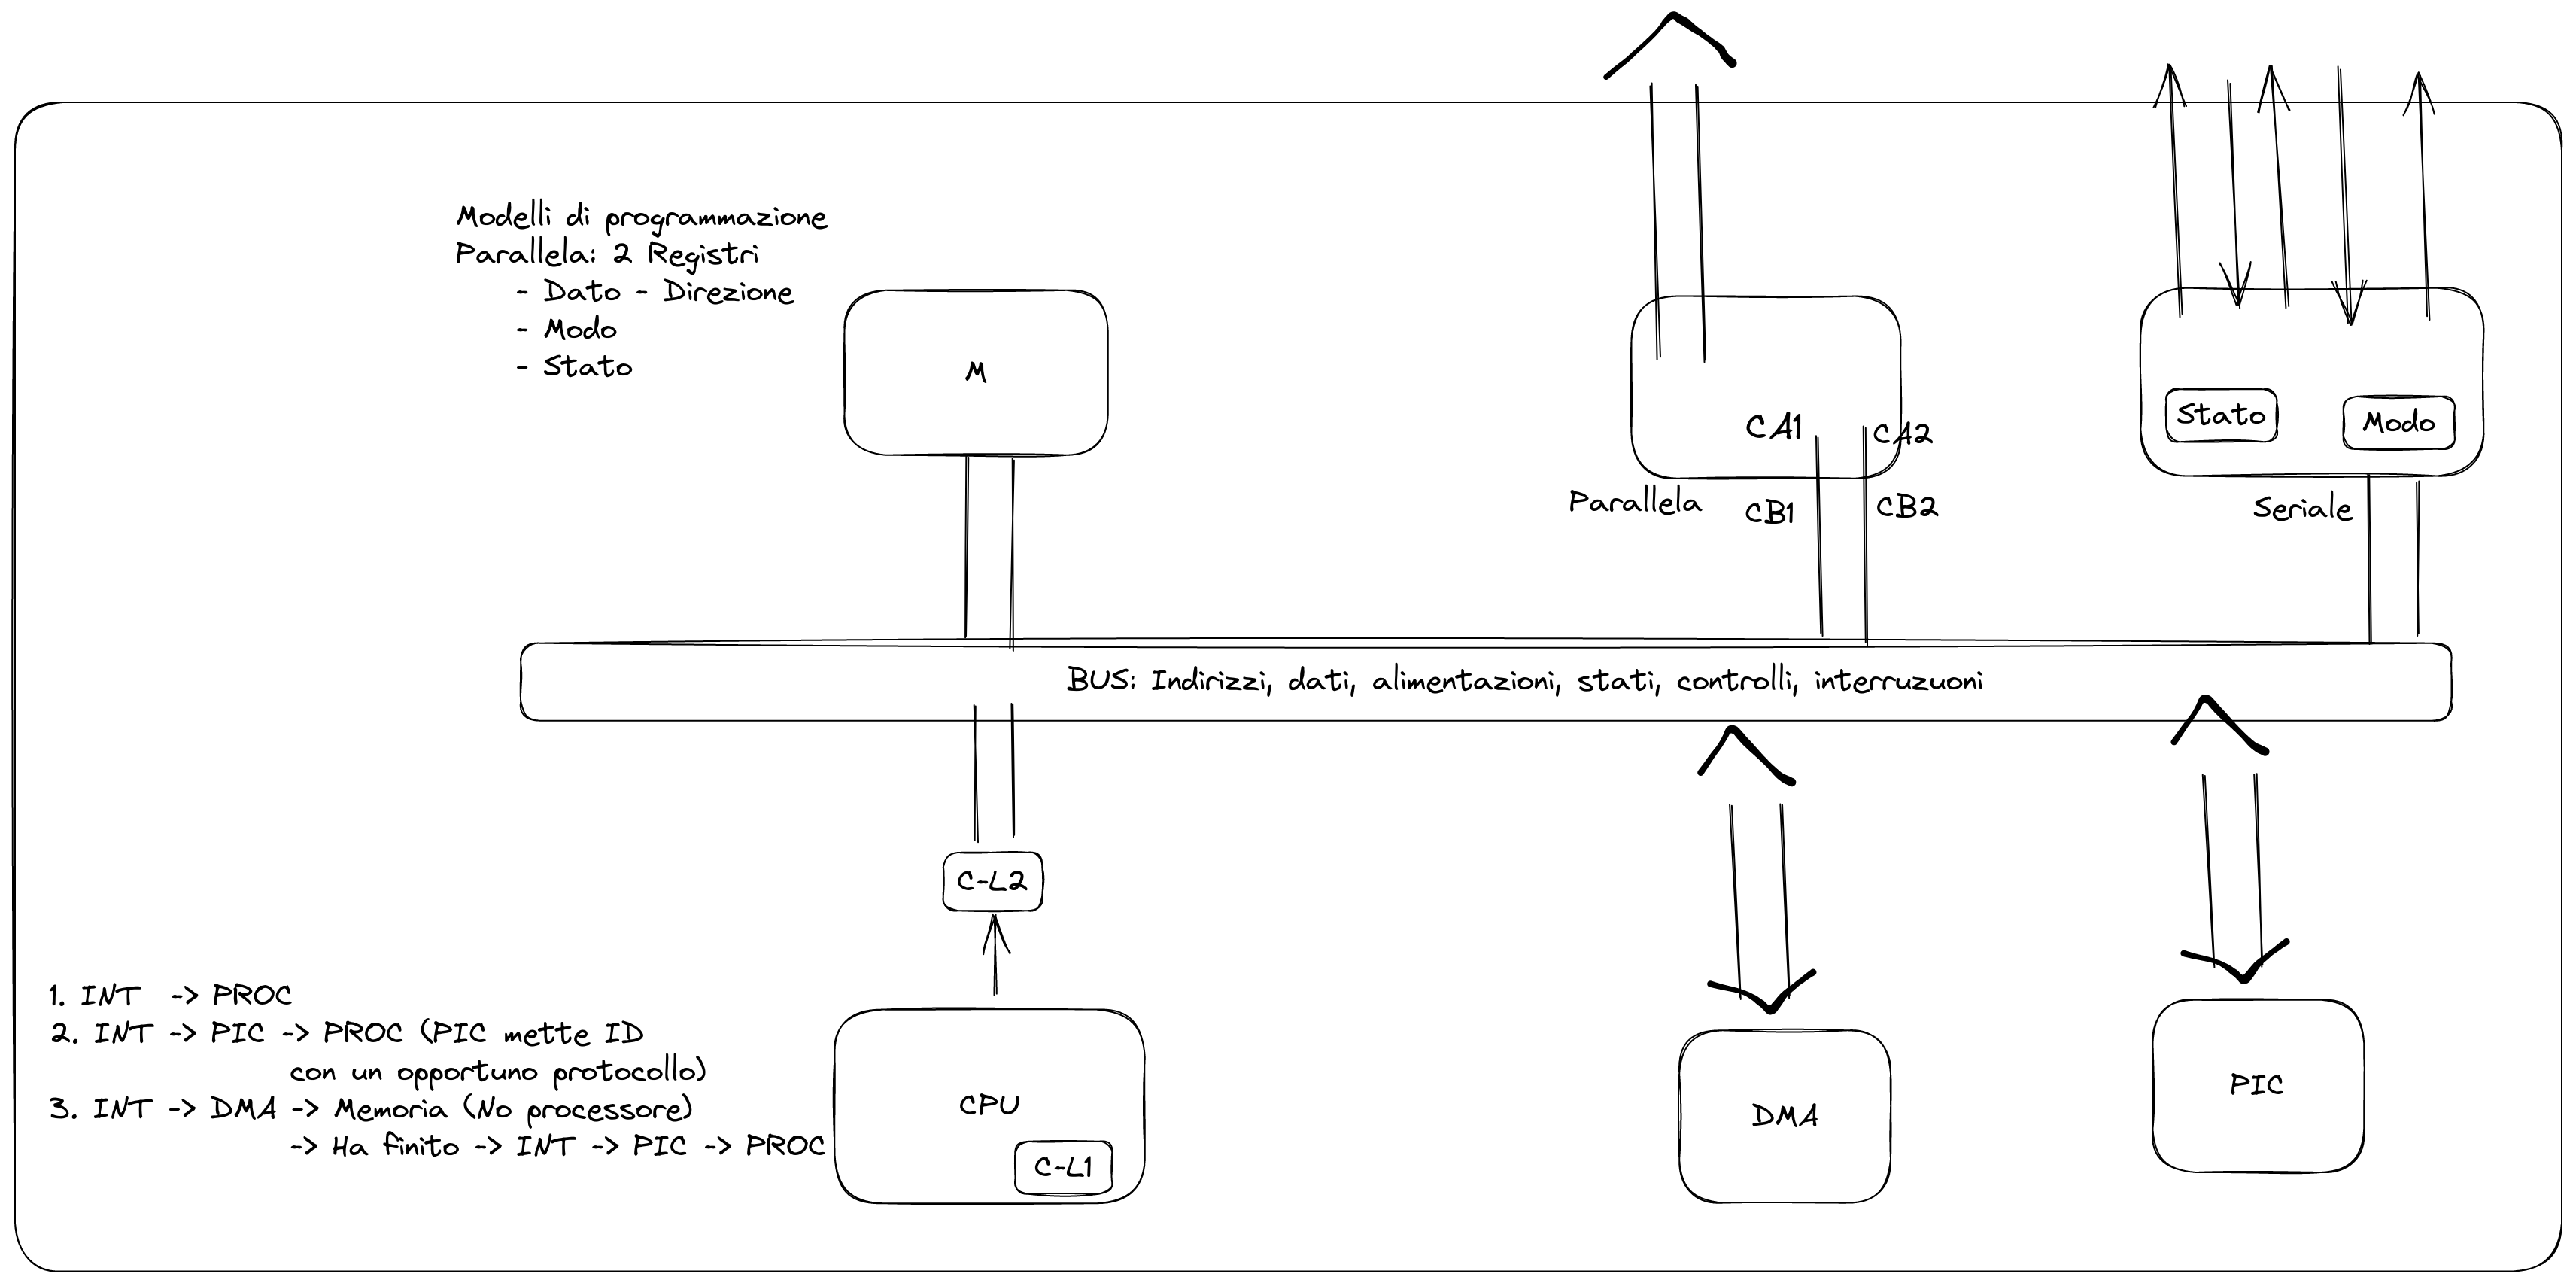
\includegraphics[scale=0.5,width=1\textwidth]
    {images/es_sistema.png}
  \caption{Esercizio completo}
  \label{fig:es_sistema}
\end{figure}

\section{PIC: Programmable interrupt controller}
\subsection{Modello di programmazione}
Il pic accetta due tipi di comandi dalla CPU: inizializzazione 
e operazione:
- inizializzazione (Initialization Command Words) (ICWs):
- operazione (Operation Command Words):

La prima operazione di inizializzazione è ICW1 (configurazione  
del numero di bit per indirizzi e modalità singola o in cascata)
, poi segue ICW2 (configurazione indirizzo base del vettore degli 
interruzioni). Le ICW3/4 sono informazioni che vengono date per configurazione 
in cascata o più complicate.

Dopo aver configurato, è possibile effettuare azioni operative. 
- OCW1: reset/set i bit della maschera delle interruzioni;
- OCW2: funzionamento del dispositivo (end of interrupt automatico o manuale);
- OCW3: special mask mode (disabilita uno specifico livello di interruzione 
senza quelli superiori o inferiori);

\section{DMA: Direct Memory Access}
Evita che il processore venga interrotto dalla periferica facendone le veci.
Il DMA ha bisogno:
- indirizzo base di memoria dove salvare il dato letto dalla periferica;
- numero di caratteri totali da leggere. Questo sarà sommato all'indirizzo 
base;
Le operazioni di configurazione delle periferica e del DMA (non può farle) vanno
fatte dal processore. Il DMA e il processore non devono avere conflitto sul bus.
In particolare, il DMA fa una richiesta al processore che deve essere accettata.
La richiesta è di tipo hardware (non interrompe il processore) può essere di due tipi:
- Ogni volta che ne ha bisogno;
- Il DMA fa una prelazione del bus (ibernando il processore che potrebbe 
continuare ad operare grazie alla cache) preoccupandosi di liberare il bus dopo 
aver finito di usarlo;
Il memory buffer nel caso dell'I/O si trova sempre nella periferica, mentre 
il memory address (nel caso dell'utilizzo del DMA) si trova nel DMA stesso, ma 
si troverebbe nel processore in architetture senza DMA. La memoria non sa se 
l'architettura prevede o meno nel DMA.\\ 
Queste operazioni creano problemi di coerenza della cache. Esistono due tecniche 
\textit{write through} e \textit{write back}. Prima di avviare il DMA, il
processore deve effetttuare il \textit{flush} della cache. Questa operazione 
è necessaria ogni volta che il DMA finisce di leggere dalla periferica.

\subsection{Intel 8237}
Ha 4 canali a cui possono essere collegate altrettante periferiche. Il canale 
rappresenta anche la priorità data alla periferica (3 priorità massima).
Funziona in 4 modalità (block, single, demand, cascade).

\end{document}


